\documentclass[a4paper,pdf]{article}
% nicer tables
\usepackage[table]{xcolor}
\usepackage{color}

% math symbols and rightarrow etc
\usepackage{graphicx}
\usepackage{amssymb}
\usepackage{amsmath}
\usepackage{centernot}
\usepackage{url} 
\usepackage[english]{babel}
% figures next to each other
\usepackage{mwe}

% checkmarks and crosses for table
\usepackage{pifont}% http://ctan.org/pkg/pifont
\newcommand{\cmark}{\color{green}{\ding{51}}}%
\newcommand{\xmark}{\color{red}{\ding{55}}}

% math symbols
\newcommand{\CI}{\mathrel{\perp\mspace{-10mu}\perp}}
\newcommand{\nCI}{\centernot{\CI}}
\newcommand{\notCI}{\not{\CI}}
\newcommand{\dsep}{\perp_d}
\newcommand{\dcon}{\not \perp_d}
\newcommand{\Dsep}{\perp_D}
\newcommand{\Dcon}{\not \perp_D}
\newcommand\causes{\dashrightarrow}
\newcommand\notcauses{\text{${}\not\!\dashrightarrow{}$}}
\newcommand\B[1]{\textbf{#1}} % bold
\newtheorem{definition}{Definition}

% For drawing graphs
\usepackage{tikz}
\usetikzlibrary{arrows}
\tikzstyle{var}=[circle,draw=black,fill=white,thin,minimum size=18pt,inner sep=0pt]
\tikzstyle{varh}=[circle,draw=gray,fill=white,thin,minimum size=18pt,inner sep=0pt,dashed]
\tikzstyle{arr}=[->,>=stealth',draw=black,thick]
\tikzstyle{arrh}=[->,>=stealth',draw=gray,thick,dashed]

\newcommand{\Sara}[1]{{\color{blue} Sara: #1}}

\begin{document}

\begin{center}

\vspace{2.5cm}

% [CHANGE] The title of your thesis. If your thesis has a subtitle, then this
% should appear right below the main title, in a smaller font.
\begin{Huge}
Applying Joint Causal Inference to a real-world biological dataset
\end{Huge}

\vspace{1.5cm}

% [CHANGE] Your full name. In case of multiple names, you can include their
% initials as well, e.g. "Jan G.J. van der Wegge".
Alex A. Khawalid\\
% [CHANGE] Your student ID, as this has been assigned to you by the UvA
% administration.
10634207

\vspace{1.5cm}

% [DO NOT CHANGE]
Bachelor thesis\\
% [CHANGE] Whether your Bachelor thesis is 6 ECTS (regular) or 9 ECTS (Honours
% programme).
Credits: 18 EC
\vspace{0.5cm}

% [DO NOT CHANGE] The name of the educational programme.
Bachelor Opleiding Kunstmatige Intelligentie

\vspace{0.25cm}

% [DO NOT CHANGE] The addess of the educational programme.
University of Amsterdam\\
Faculty of Science\\
Science Park 904\\
1098 XH Amsterdam

\vspace{4cm}

\emph{Supervisor}\\
% [CHANGE] The name of your supervisor. Include the titles of your supervisor,
% as well as the initials for *all* of his/her first names.
Sara Magliacane

\vspace{0.25cm}

% [CHANGE] The address of the institute at which your supervisor is working.
% Be sure to include (1) institute (is appropriate), (2) faculty (if
% appropriate), (3) organisation name, (4) organisation address (2 lines).
%Institute for Language and Logic\\
Institute of Informatics\\
Faculty of Science\\
University of Amsterdam\\
Science Park 904\\
1098 XH  Amsterdam

\vspace{1.5cm}

% [CHANGE] The date at which you will finalize and submit your thesis.
July 2nd, 2017

\end{center}

\newpage

\section*{Summary}
Joint Causal Inference (JCI) \cite{jci} is a recently proposed causal discovery framework that aims to discover causal relations based on multiple observational and experimental datasets, also in the presence of hidden variables. Currently, JCI has only been tested on simulated data and is mostly applicable to systems with a small number of variables. To circumvent this issue, a simplified version of JCI, non-deterministic JCI, was designed. This thesis applies non-deterministic JCI to two standard causal discovery algorithms, GFCI and FGES \cite{gfci}. Subsequently, it evaluates the performance of its approaches on simulated data, generated using a simulator from literature \cite{jci}. The evaluation suggests that implementing non-deterministic JCI improves the performance of the predicted causal relations with respect to  previous approaches, especially in combination with bootstrapping standard causal discovery methods. Finally, this research applies its approach to a real-world biological dataset  \cite{sachs2005causal}, showing consistent results to other types of methods.

\newpage
%\section{Contents}
\tableofcontents

\newpage
\section{Introduction}
When examining data in the field of statistics, occasionally a correlation may occur between two events that seem unlikely to be related in any way. When these correlations are discovered, they are sometimes mistaken as a causal relation between these two events. 
One case which is commonly used to illustrate this situation, is the chocolate consumption and Nobel laureates correlation. In a research conducted in 2012 by Franz H. Messerli \cite{nobelchocolate}, a correlation between chocolate consumption per capita and Nobel laureates per ten million people in a country was discovered, as illustrated in Figure \ref{fig:choc}.

\begin{figure}[!ht]
    \centering
    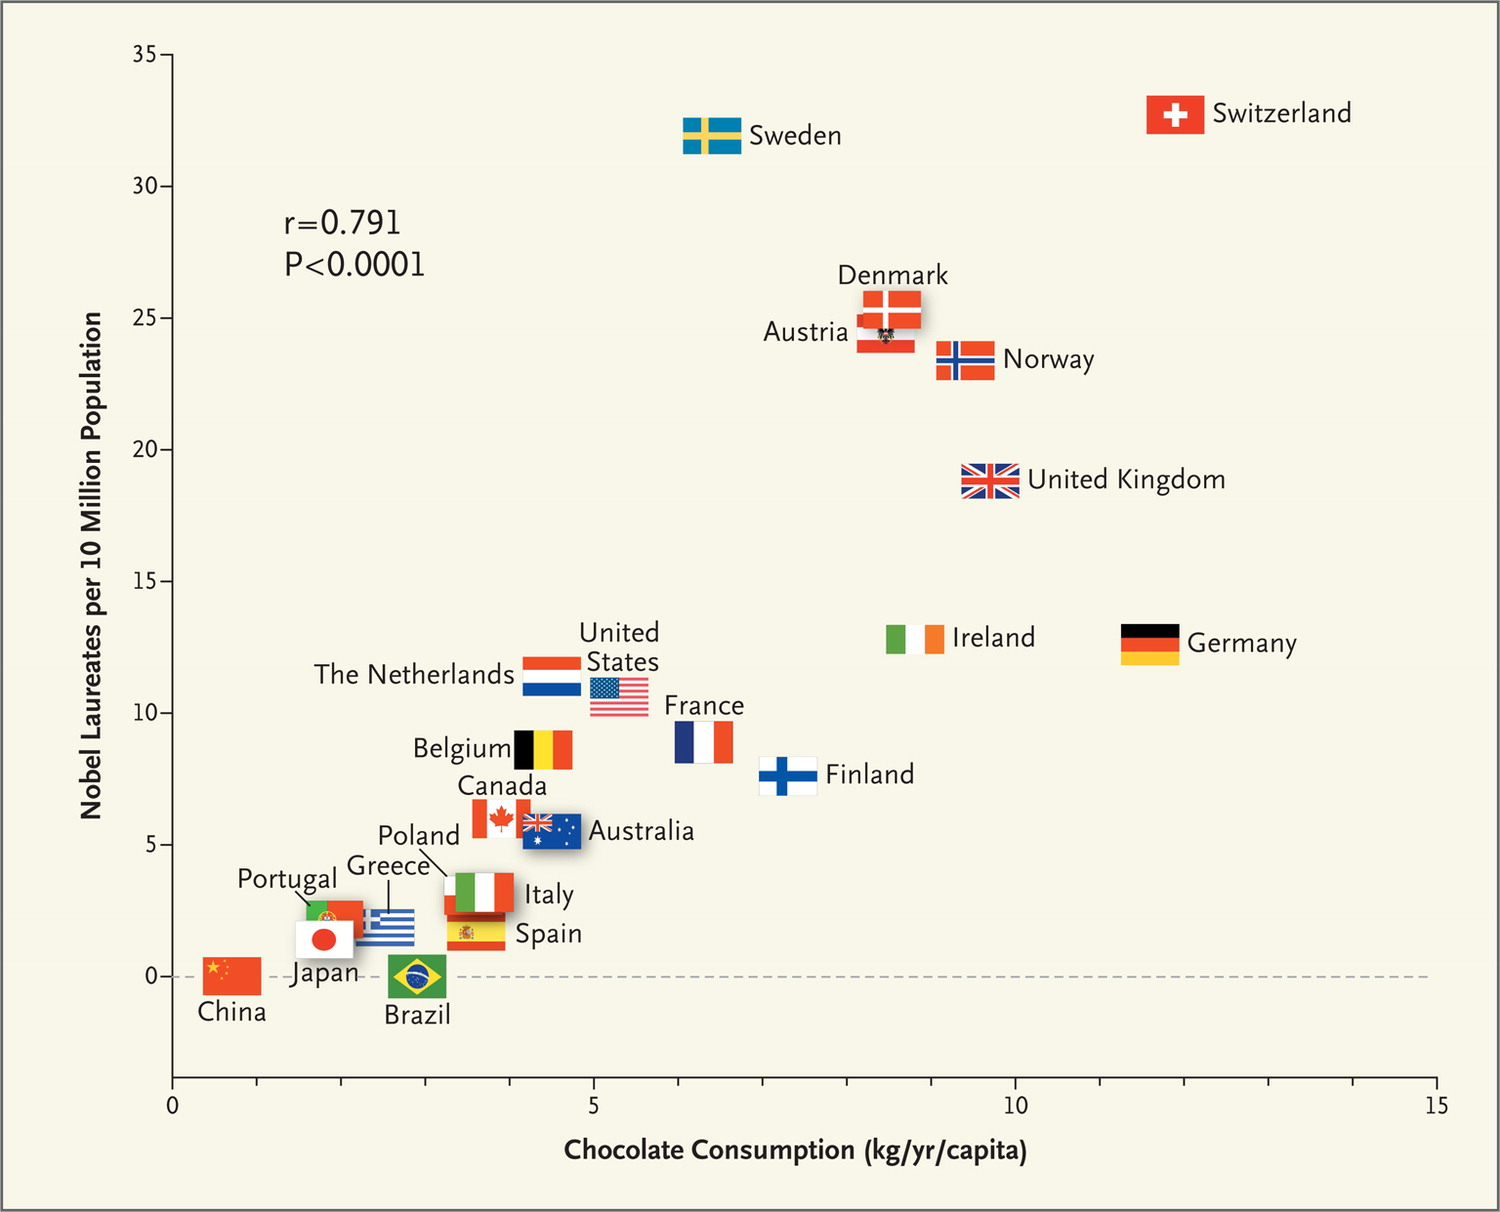
\includegraphics[width=\textwidth]{chocolate}
    \caption{The number of Nobel laureates per 10 million people in a country and the annual chocolate consumption per capita, as illustrated in a paper by Franz H. Messerli \cite[p.~1563]{nobelchocolate}}
    \label{fig:choc}
\end{figure}
Although it is difficult to prove, it is highly unlikely that eating more chocolate would cause a country to have more Nobel laureates. A more likely explanation is that chocolate consumption and increased number of Nobel laureates per 10 million people could be a result of financial stability in these countries. 

As shown by this example, `correlation is not causation', i.e. correlation indicates a connection between two events, but this connection is not necessarily of a causal nature. 
While it is true that a correlation is not sufficient to prove a causal relation, it is wise to research what does imply causation. Causal discovery \cite{Pearl2009inference,Spirtes2000} is a field of statistics that tries to find methods to uncover these causal relations.

Within the field of causal discovery, a number of different methods exist. These methods generally attempt to reconstruct the causal structure underlying the data from the data itself. 
Usually, methods can be classified in two categories; score-based methods and constraint-based methods. Ordinarily, score-based methods rate the possible causal structures and assume that the best scoring structure represents the causal structure underlying the data. Constraint-based methods use certain assumptions to eliminate some of the possible causal structures. As opposed to score-based methods, these methods can tolerate the presence of latent variables in a system, such as financial stability in the chocolate correlation, which is often the case in real-world applications.

Joint Causal Inference (JCI) \cite{jci} is a recently proposed constraint-based framework that aims to discover causal relations based on multiple observational and experimental datasets. Similar to other causal discovery methods, the overall goal of JCI is to find causal relations without extensive experimentation. This will enable more purposeful and less expensive research in some fields, for example biology.
%Currently, JCI has only been tested on simulated data and is mostly applicable to systems with a small number of variables. 

While JCI predicts causal relations more accurately than standard methods on these simulated datasets, several open questions remain. This thesis aims to answer the following research question:
\begin{quote}
\textbf{Research question 1}: How does Joint Causal Inference perform on real-world datasets?
\end{quote}
Unfortunately, one cannot apply the current version of JCI to most real-world datasets, because of its limitation to a small number of variables. The main reason for this limitation is that JCI can only be used in combination with certain methods, because the deterministic relations introduced by JCI are problematic for most causal discovery methods. So, another important research question that this thesis tries to answer is:
\begin{quote}
\textbf{Research question 2}: How can one implement a simplified version of Joint Causal Inference that scales up to the number of variables in a real-world dataset?
\end{quote}
In this thesis, some answers are provided to these research questions by designing and implementing a simplified version of JCI that allows for the use of most established methods for causal discovery. 
The main idea of this simplified approach is to avoid introducing problematic deterministic relations.
This research combines this approach and two other standard causal discovery methods, Fast Greedy Equivalence Search (FGES), a well-established method in literature, and Greedy Fast Causal Inference (GFCI) \cite{gfci}, a newly developed causal discovery method that combines FGES and another important causal discovery method, Fast Causal Inference (FCI) \cite{Spirtes2000}.

The implementation produced for this thesis will be evaluated on a simulated dataset, this will demonstrate its accuracy. Subsequently, this thesis applies its method to a protein signalling network dataset \cite{sachs2005causal} that is often used to benchmark different causal discovery methods, showing its potential for real-world causal discovery.

\newpage
\section{Background: Causal Discovery}
Causal discovery, the cornerstone of this research, is a field in statistics with a rich history, as described in more detail in ``Causal Inference in Statistics: A Primer''  \cite{pearlprimer}. Causal discovery aims to uncover causal relations between random variables. In this context, a causal relation ``X causes Y'' is a relation where an intervention (or manipulation of the value of a random variable) that changes a random variable X, changes the distribution of the random variable Y as well \cite[p.~5]{pearlprimer}. 

Causal relations can be described with sets of equations called Structural Causal Models that will be summarised in Section \ref{sec:scm}. These equations can also be represented by causal graphs. The methods that will be presented in this thesis, will generate causal graphs based on a dataset.
Generating accurate graphs for underlying causal structures requires a basic understanding of graph theory, which will be presented in Section \ref{sec:basic_graph}. 

\subsection{Structural Causal Models}\label{sec:scm}
\begin{figure}[!ht]
    \centering
    \renewcommand{\arraystretch}{2}
    \setlength{\tabcolsep}{7pt}
    \rowcolors{2}{blue!10}{blue!15}
    \begin{tabular}{|c|c|l|}
        \multicolumn{3}{c}{\large{\textbf{Structural Causal Model (SCM)}}}\\
        \hline
        \textbf{U}&$\{X\}$&Set of exogenous variables\\ \hline
        \textbf{V}&$\{Y \}$&Set of endogenous variables\\ \hline
        \textbf{F}&$\{f_Y: Y = 6X \}$&Set of functions to determine values for V\\
        \hline
    \end{tabular}\\
    \caption{An example of an SCM \label{fig:sub1}}
\end{figure} 
Modelling a variable and its causes might seem like a difficult task. Some method has to be used to make such a task manageable. One such method is describing these variables within a structural causal model (SCM) \cite[p.~26]{pearlprimer}. A SCM uses two sets of variables and a set of functions to describe variables and the relevant features of the setting in which these variables occur, as summarised in Figure \ref{fig:sub1}. These two sets of variables, U and V, are exogenous variables and endogenous variables respectively. Exogenous variables are not a part of the model, their causes are not modelled. Endogenous variables are a part of the model, their causes are modelled. The set of functions F, is used to describe the relation between the variables in the model.
 


\subsection{Basic graph theory} \label{sec:basic_graph}
% basic graphs, edges, nodes, adjacency, path, d-separation 
SCMs can be described by causal graphs, which is the type of output nearly all methods for causal discovery use. A causal graph is a graphical representation, it contains nodes (representing random variables) and edges (representing causal relations). 
An edge $X\to Y$ from a node X to a node Y in the graph represents a direct causal relationship of cause $X$ on effect $Y$. 
Two nodes are adjacent if they are connected by an edge. A path is available between two nodes, as long as there is a series of adjacent nodes connecting them. If all edges in a given path are directed, e.g. $X_1 \to X_2 \to \dots \to X_n$, the path is a \emph{directed path}.
If there is a directed path from $X$ to $Y$ then $X$ is an \emph{ancestor} of $Y$, which one writes as $X \causes Y$. Otherwise one says that $X \notcauses Y$.

This thesis focuses on causal graphs without cycles, which are also called Directed Acyclic Graphs, or DAGs. These DAGs are a useful tool when representing the underlying structures from a dataset. Some combination of paths (or absences of paths) in DAGs have important consequences for causal discovery and are described by a criterion called \emph{d-separation} \cite{Pearl2009inference,Spirtes2000}, defined as:
% D-separation is not a requirement but a description of certain combinations of path. It doesn't require that something happens, it just describes it. The requirements are all in the Causal Markov and faithfulness assumptions. So, I changed a bit the above part.

\begin{definition}
  For disjoint sets of variables $X,Y,\B{W}$ in a DAG, one says that $X$ is d-separated from $Y$ by $\B{W}$, denoted as $X \dsep Y | \B{W}$, if and only if every path $\pi$ that connects $X$ with $Y$ is \emph{blocked} by $\B{W}$, i.e. at least one of the following holds:
  \begin{itemize}
    \item $\pi$ contains a collider $C$ (a node on the path that has two incoming arrow heads) that is caused by $\B{W}$ ($\B{W} \causes C$), or
    \item $\pi$ contains a non-collider in $\B{W}$.
  \end{itemize}
  Otherwise, one says that $X$ and $Y$ are d-connected given $\B{W}$, or $X \dcon Y | \B{W}$.
\end{definition}
  
% basic graph showing x -> y
\begin{figure}[!ht]
    \centering
    \begin{minipage}{0.45\textwidth}
        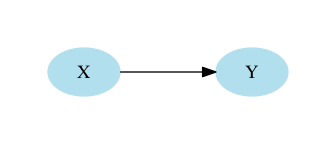
\includegraphics[width=\textwidth]{basiccause}
        \caption{Two variables X and Y, where X causes Y, illustrated in a simple causal graph. For example, X could be the temperature outside and Y could be your desire to eat ice cream. \label{fig:basiccause}}
    \end{minipage}\hfill
    \begin{minipage}{0.45\textwidth}
        \centering
        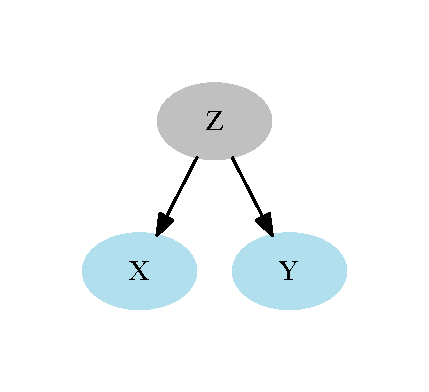
\includegraphics[width=\textwidth]{commoncause}
        \caption{Two variables X and Y, where X and Y are influenced by a latent confounder Z, illustrated in a causal graph. For example, X could be the chocolate consumption per capita and Y could be the number of Nobel Laureates. In this case the latent confounder could be financial stability.\label{fig:latentconfounder}} 
    \end{minipage}
\end{figure}

The SCM in Figure \ref{fig:sub1} could also be illustrated as a graph. One possible graph that could represent this SCM is shown in Figure \ref{fig:basiccause}. The causal graph shown in Figure \ref{fig:latentconfounder} is another example of a DAG, in this example the variable Z is an unmeasured variable. 



% how are relations obtained?
In causal discovery, there are often two types of data, observational data and experimental data. In certain circumstances, variables can behave differently than in others. To see what type of reaction these variables have in these circumstances, interventions are applied. The data resulting from these interventions is referred to as experimental data. Data where no interventions are applied is referred to as observational data.

% intervention
Applying an intervention in a causal discovery context means to manipulate the value of certain variables within a model. Depending on the type of intervention used, this could mean to control their value completely, but also to inhibit or stimulate their value. A soft intervention is an intervention which only inhibits or stimulates the value of a certain random variable. Contrarily, a perfect intervention is an intervention which can control the value of a targeted variable exactly. Interventions can be used to examine the way other variables react to these values. However, in most cases applying an intervention is either hard, expensive, or both. This means a limited amount of experimental data is available for a number of situations which concern causal discovery.


\subsection{Reichenbach's principle}
Occasionally, a correlation between two variables X and Y occurs, and sometimes the relation between these variables is not of a causal nature. Reichenbach's principle \cite{Reichenbach1956}, also known as the common cause principle, is the idea that when the aforementioned situation takes place, one of or some combination of the following statements about this relation must be true:\\
\begin{itemize}
    \item X causes Y
    \item Y causes X 
    \item there is a common cause for X and Y
\end{itemize}

Considering this, correlation does provide some evidence of a relation between two correlated variables. The nature of these connections can be revealed, provided sufficient data, by causal discovery methods.
% \Sara{Try to connect Reichenbach's principle with the next section, for example say that to give an idea that correlation can give some evidence about causation.}

\subsection{Causal Discovery}
There are two categories of causal discovery; score-based and constraint-based. Joint Causal Inference \cite{jci}, the main framework that will be discussed in this thesis, is part of the constraint-based category of causal discovery. As opposed to score-based methods, these methods allow for the presence of latent variables in a system, which is often the case in real-world applications.

Constraint-based causal discovery usually relies on a few assumptions. The two main assumptions are the causal Markov assumption and the faithfulness assumption \cite{fci,jci}, which together define the correspondence between statistical independences and combinations of edges in the graphs. Using these assumptions, a causal graph can be constructed from the results of the statistical independence tests in the data. The causal Markov assumption is described as follows: ``\textit{d-separation in the causal DAG $\mathcal{G}$ implies conditional independence in the observational distribution $\mathcal{P}$}'' \cite[p.~3]{jci}. This holds for all disjoint sets of variables \textbf{X}, \textbf{Y}. The faithfulness assumption is the inverse of the causal Markov assumption. These two assumptions can more formally be represented by the following formulas:
\begin{itemize}
    \item \textbf{Causal Markov Assumption:} $$\textbf{X} \dsep \textbf{Y} | \textbf{W}[\mathcal{G}] \Longrightarrow \textbf{X} \CI \textbf{Y} | \textbf{W}[\mathcal{P}]$$
    \item \textbf{Faithfulness Assumption:} $$\textbf{X} \nCI \textbf{Y} | \textbf{W}[\mathcal{P}] \Longrightarrow \textbf{X} \dcon \textbf{Y} | \textbf{W}[\mathcal{G}] $$
\end{itemize}
Where \textbf{X,Y,W} are disjoint sets of variables, $\dsep$ stands for d-separated and $\CI$ stands for conditionally independent, as opposed to d-connected $\dcon$ and conditionally dependent $\nCI$. 
%\Sara{This is not true: $\textbf{W}$ is the set of ancestors of any variable for which $X \not \rightarrow \textbf{W}$ given $X \not \rightarrow Y$ for all $Y \in \textbf{W}$}
% conditioning on nodes

Conditional independence tests are very important to constraint-based methods in causal discovery. These tests examine the effect conditioning upon certain variables has on causal relations.  Conditional independence between variables X and Y, conditioned upon variable Z is denoted as $X \CI Y | \B{Z}$. Informally, this means that given the value of Z, the values X and Y do not determine each others values. An example of this, taken from ``Conditional Independence'' \cite{wiki:CI}, is that height and vocabulary of a person sampled from some population are not independent. However when conditioning upon age, they are conditionally independent.% Trying to give a more intuitive understanding of conditional independence 

	
%\section{Literature Review}
\section{Background} 
Among the constraint-based causal discovery methods, there are a few that are related to the work presented in this thesis. This section summarises them, and then introduces the background of the thesis, Joint Causal Inference.

Ancestral Causal Inference (ACI) \cite{aci} is a recently developed constraint-based method that produces similarly accurate results to other state of the art methods, but with lower running times. ACI produces an ancestral structure, which is a set of indirect causal relations. 
% a Markov equivalence is a very specific type of class of graphs, which are the ones that have the same conditional independences, an ancestral structure is if you prefer a transitive equivalence class, but it seems overly complicated
Using ancestral structures is one of the factors that allow it to run faster than similar methods with different representations by orders of magnitude. 

Local Causal Discovery (LCD) \cite{cooper1999causal} is a constraint-based method that discovers causal relations for a simple causal pattern. Compared to ACI, the LCD method is better equipped to exploit the information from multiple observational and experimental datasets, but it can only use a limited amount of information from independence tests.

Using the concepts discussed in the previous sections, the primary focus of this research, Joint Causal Inference (JCI) \cite{jci}, will be discussed. JCI is a framework used to discover causal relations from multiple observational and experimental datasets, that extends the ideas from LCD and the score-based approach by Eaton and Murphy \cite{eaton2007exact}. JCI contains a different set of assumptions which enables methods to use multiple datasets to generate a general underlying causal graph across all of the datasets. Standard causal discovery methods cannot be applied to JCI because of faithfulness violations, which are caused by deterministic relations from JCI. These problems are solved using an extension of ACI called Ancestral Causal Inference with Determinism (ACID). 
Similarly to ACI, the output model is an ancestral structure. ACID-JCI has successfully been tested on simulated data. One of the issues of ACID-JCI is the scalability of the method. Specifically, the method runs in a reasonable time only for a handful of variables, while many real-world problems are more complex. 

Because of these limitations, this thesis will focus on a simplified version of JCI that removes the deterministic relations, which are problematic for most current constraint-based causal discovery methods.
This version of JCI can be solved with standard methods, optionally by adding some of the JCI background knowledge. This will allow one to scale much more than with the ``full'' version of JCI and apply these methods to a real-world dataset by Sachs et al. \cite{sachs2005causal}.

This paper describes the dataset which will be used and is necessary to understand it.  The dataset contains data about protein concentrations after adding certain drugs, that act as inhibitors or activators of certain proteins. The purpose of applying JCI to such biological datasets is to uncover causal relations in cell signalling networks. Gaining more insight into these cell signalling networks will help in treating diseases more effectively. Understanding cell signalling networks shows how cells react to their environment and how they decide what actions to take.

\section{Approach: Non-deterministic JCI} 
\begin{figure*}[!ht]

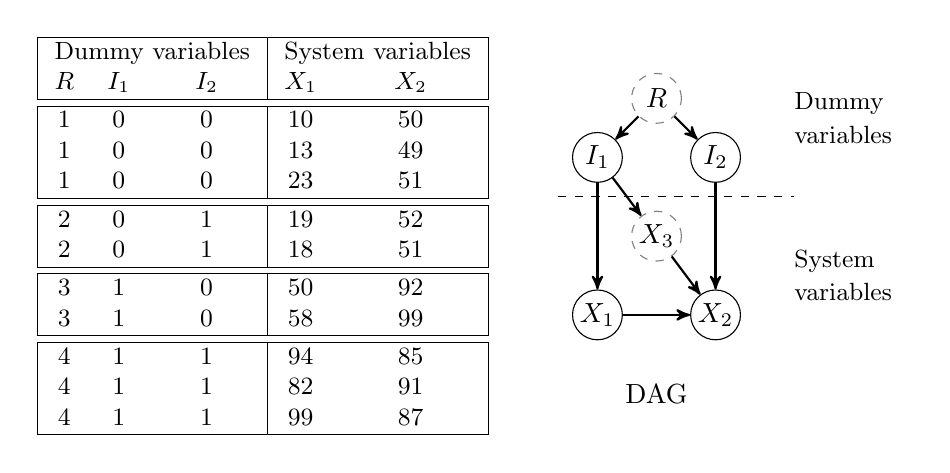
\begin{tikzpicture}
\begin{scope}[xshift=0cm]
  \node at (0,-0.5) {\small\begin{tabular}[t]{|ccc|cc|}
    \hline
    \multicolumn{3}{|c|}{Dummy variables} & \multicolumn{2}{c|}{System variables} \\
    $R$ & $I_1$  & $I_2$ & $X_1$ & $X_2$\\
    \hline
    \hline
    1 &  0 & 0 & 10  & 50\\
    1 &  0 & 0 & 13 & 49\\
    1 &  0 & 0 & 23 & 51\\
    \hline
    \hline
    2 &  0 & 1 & 19 & 52\\
    2 &  0 & 1 & 18 & 51\\
    \hline
    \hline
    3 &  1 & 0 & 50 & 92\\
    3 &  1 & 0 & 58 & 99\\
    \hline
    \hline
    4 &  1 & 1 &  94 & 85\\
    4 &  1 & 1 &  82 & 91\\
    4 &  1 & 1 &  99 & 87\\
    \hline
  \end{tabular}};
\end{scope}
\begin{scope}[xshift=5cm,yshift=0.5cm]
  %Nodes
  \node[varh]        (R)       at (0,0.75) {$R$};
  \node[var]      (I1)        at (-0.75,0) {$I_1$};
  \node[var]      (I2)        at (0.75,0) {$I_2$};
  \node[var]        (A)       at (-0.75,-2)  {$X_1$};
  \node[var]        (B)       at (0.75,-2) {$X_2$}; 
  \node[varh]        (D)      at (0,-1) {$X_3$}; 
   
  \draw[dashed] (-1.25,-0.5) -- (1.75,-0.5);
  \node at (0,-3) {DAG};
  \node[text width=1.5cm] at (2.5,0.5) {\small Dummy variables};
  \node[text width=1.5cm] at (2.5,-1.5) {\small System variables};
  %Lines
  \draw[arr] (R) edge (I1);
  \draw[arr] (R) edge (I2);
  \draw[arr] (I1) edge (A);
  \draw[arr] (I2) edge (B);
  \draw[arr]  (I1) edge (D);
  \draw[arr] (A) edge (B);
  \draw[arr] (D) edge (B);
\end{scope}
\end{tikzpicture}
%\end{topalignedcolumn}
\caption{This figure illustrates a case where JCI is applied, similar to the example from Magliacane et al. \cite{causalTransfer}. In this context there are 4 datasets with two interventions, $I_1$ and $I_2$. The table on the left demonstrates JCI as applied in this context. The DAG on the right shows the true model underlying the datasets and a latent system variable $X_3$. An example of a system being modelled could be exam performance. The intervention variables could represent different methods of studying and the system variables could represent performance on exams out of 100. The latent system variable $X_3$ could represent interest in a subject.\label{fig:JCI_example}}
\end{figure*}
% \Sara{In practice JCI is not really explained before, so I don't know if the following is enough to understand what does the method do. I have added an image from an unpublished paper \cite{causalTransfer} that could maybe help explain the concept.  I added also an interpretation similar to the Sachs dataset, if you want you can change it.

% The main idea of non-det JCI is to use all datastets together and add the intervention variables (which is not the usual way of modelling interventions and works only for soft interventions). Then under certain assumptions, e.g.}

% what does jci do?
The principal idea of non-deterministic JCI is enabling the use of all of the datasets in the same method as well as adding intervention variables. In general, most methods do not allow for the use of multiple datasets. Neither do these methods enable learning the target of interventions, although it is essential to note that learning these targets can only be done when these interventions are soft interventions. Figure \ref{fig:JCI_example} shows an example of the application of JCI. 

% what is jci?
Within the JCI framework there are two sets of variables, a set of dummy variables and the system variables. The set of dummy variables contains the regime variables and the intervention variables, denoted as $R$ and $I_n$ respectively for the example in Figure \ref{fig:JCI_example}. The system variables are the set of all variables being modelled. Each dataset is assigned a regime variable indicating which experimental setting it belongs to, these regime variables are deterministically related to the intervention variables. For every experimental setting the interventions that have been applied in this setting are marked as 1 for the corresponding intervention variables. In all other settings they are marked as 0. An example of this is also depicted in Figure \ref{fig:JCI_example}.

% why ndJCI?
The ``full'' JCI framework has some problems, such as deterministic relations and scalability, which were discussed in the previous sections. In light of these problems, a simplified version of JCI was determined to be more appropriate. This simplified version of JCI, non-deterministic JCI, will accommodate the use of a variety of causal discovery methods. This was deemed to be important, as it enables the use of more efficient methods by allowing its use in a non-deterministic setting. These efficient methods, that only work in a non-deterministic setting, will be more easily applicable to the data set.

% Non-deterministic JCI will allow the use of a number of causal discovery methods by discarding the regime variable. Certain elements which caused deterministic relations were removed from the framework. This simplified framework is the result.

% how does ndjci work?
Non-deterministic JCI requires a specific set of steps to function properly. Within the non-deterministic JCI framework, the regime variables are discarded after creating the intervention variables. To create a non-deterministic setting, this must be done as the regime variables have a deterministic relation with the intervention variables.
These intervention variables cannot have a deterministic relation with each other, this enables methods to be used without violating the faithfulness assumption. Once these intervention variables have been non-deterministic set up, the framework should add background knowledge to the methods if possible. The following statements should be included in the background knowledge:
\begin{itemize}
    \item \textit{No variables can cause an intervention variable, neither system variables nor intervention variables}
    \item \textit{Latent confounders cannot cause both system variables and intervention variables}
\end{itemize}

\section{Implementing non-deterministic JCI}
The primary focus of this research is to apply non-deterministic JCI to a real-world dataset. Examining the results of this application will reveal how JCI performs in a real-world setting, as well as demonstrating the fact that JCI can be scaled to a larger set of variables.

Since a large collection of libraries and tools are available for causal discovery in R, this thesis will make use of this collection and the resulting system will be written in R. The main package that will be used is the rcausal package \cite{r-wrapper}, which will enable the use of the Tetrad system \cite{tetrad}. The Tetrad system contains numerous different methods for causal discovery. This research will focus on the FGES and GFCI methods, and apply them to non-deterministic JCI. 

Simulated data will be used to demonstrate the effect of certain aspects of the non-deterministic JCI framework on the performance of the methods used in this research. This simulated data will be generated by a method from the aci package \cite{jci}. Furthermore, the evaluation of the performance of these methods will be assessed using ROC curves. These curves will also be generated by code from the aci package \cite{jci}. 

\subsection{Preprocessing datasets for non-deterministic JCI}
Among the assumptions made by non-deterministic JCI, is the assumption that no deterministic relations between the intervention variables can exist.
In the real-world dataset on which the method is applied, the Sachs dataset \cite{sachs2005causal}, some of the interventions are determined by others. So before applying non-deterministic JCI, the deterministic relations were found and removed by hand. The result of this can be found in Table \ref{tab:ndjci}.


\begin{table}[!ht]
    \centering
     \renewcommand{\arraystretch}{2}
    \setlength{\tabcolsep}{7pt}
    \rowcolors{2}{blue!10}{blue!15}
    \makebox[\textwidth][c]{\begin{tabular}{|c|c|c|c|c|c|c|c|c|c}
    \hline
    exp.&ICAM&AKT&G0076&$\Psi$tectorigenin&U0126&LY294002&PMA&$\beta$2CAMP\\
    \hline
    1&0&0&0&0&0&0&0&0\\ \hline
    3&0&1&0&0&0&0&0&0\\ \hline
    4&0&0&1&0&0&0&0&0\\ \hline
    5&0&0&0&1&0&0&0&0\\ \hline
    6&0&0&0&0&1&0&0&0\\ \hline
    7&0&0&0&0&0&1&0&0\\ \hline
    8&0&0&0&0&0&0&1&0\\ \hline
    9&0&0&0&0&0&0&0&1\\ \hline
    \hline
    2&1&0&0&0&0&0&0&0\\ \hline
    10&1&1&0&0&0&0&0&0\\ \hline
    11&1&0&1&0&0&0&0&0\\ \hline
    12&1&0&0&1&0&0&0&0\\ \hline
    13&1&0&0&0&1&0&0&0\\ \hline
    14&1&0&0&0&0&1&0&0\\ \hline
    \end{tabular}}
    \caption{Table with several datasets used in the research and the respective values of the intervention variables. All of the deterministic relations caused by the intervention variables have been removed.\label{tab:ndjci}} % Removed some columns, which are not mentioned here, like alpha CD3- and alphaCD23
\end{table}


\subsection{Adding background knowledge}
For the purpose of implementing one of the assumptions of non-deterministic JCI, the addition of prior knowledge to the methods is important. The Tetrad system allows the addition of prior knowledge by specifying the order of all of the variables into separate tiers. Within the Tetrad system this is referred to as temporal knowledge. The intervention variables were added to the first tier, and the system variables were put into a tier below them. With this addition no direct edges can go from the system variables to the intervention variables, however the contrary is possible. 
% Although this implements one of the assumptions of non-deterministic JCI, it still allows the presence of latent confounders causing both system and intervention variables.

\subsection{Applying standard constraint-based methods}
% \Sara{I think you can just use what you previously had in the background here to explain what GFCI and FGES do. It may need a bit rewriting, because I was copy pasting it around. Then it is more clear what is the approach you implemented. Maybe you can also move it before the previous section in which you talk about background knowledge.}

% explain fges and gfci
The non-deterministic JCI framework has to be applied to a specific method, as it is not a method on its own. This section will explain the workings of the two methods to which JCI was applied. The first method, GES \cite{ges}, is a score-based method which uses heuristics to search for the true graph. One of the disadvantages this method has, is that it assumes there are no latent confounders. When these latent confounders are present, it is possible GES will find adjacencies that are not present in the true graph \cite[p.~372]{gfci}. In this thesis, a specific implementation of GES, FGES \cite{ges} is used. The second method used, Greedy Fast Causal Inference (GFCI) \cite{gfci}, is a combination of Greedy Equivalence Search (GES) and FCI \cite{fci}.  

% fci works like this
FCI is a method which separates its search for a true graph in two operations. Before starting any operations, FCI assumes all nodes have undirected edges connecting them to each other. Firstly, FCI starts by ruling out direct paths from one node to another by using conditional independence tests. Secondly, after all of the adjacencies that do not belong in the graph have been removed, FCI attempts to orient all of the edges in its graph. FCI produces a partial ancestral graph (PAG), which is a structure that represents several causal graphs that are equally possible given the independence tests.

% they are combined like this in gfci
In GFCI these methods are combined as follows: the first part of FCI, the removal of adjacencies through independence tests, is performed on the results of GES. This enhances the accuracy of the algorithm by removing edges. Subsequently, the results of GES are used in directing the edges during FCI. This results in a more accurate PAG with more directed edges. Taking these facts into account, GFCI seems like an appropriate method to apply JCI to.


%It uses GES to improve the accuracy of FCI.
% Like most current constraint-based methods, FCI cannot deal with determinism without violating faithfulness assumptions, so it can be applied to a simplified version of JCI with no deterministic relations. 
%Moreover, it is much more scalable in the number of variables, making it a good candidate for a real-world application of the simplified JCI setting.

\section{Results}
This section will start by describing the evaluation of the GFCI and FGES methods with non-deterministic JCI on simulated data. After this primary evaluation, the methods were tested on real-world data, specifically data involving protein concentrations in protein signalling networks \cite{sachs2005causal}.

\subsection{Evaluation setting}
For all of the simulated datasets a true model is available. The performance of these methods can be measured using ROC curves. These are curves demonstrating the rate of true positives (the amount of correctly assessed relations) against the rate of false positives (the amount of relations incorrectly assessed as true). The area under the curves can be used as a measure of their performance. The closer these values are to one, the better. As long as the values stay above 0.5, the values are better than randomly assigning relations.  

The generally accepted model for the Sachs dataset is not fit to be used as a golden standard, as it is still not certain to be the true model. Therefore, the results of the application to real-world data will be evaluated by looking at similarities to other methods as well as the consensus model. 

Since one of the goals of this research is to examine the performance of JCI, an appropriate baseline would be the same methods without JCI. As such the methods used in combination with JCI will also be tested without it. This allows for a comparison showing the tangible effects JCI has on the performance of a method.

\subsection{Simulated data}
%  This simulated data will be generated by a method from the aci package \cite{jci}
This research uses the simulator from the code in the aci package \cite{jci}, to generate simulated data. This tool was adjusted to also work with interventions. The simulator generates data for a given number of linear acyclic models for each permutation of the variables and the interventions given to the simulator. The models have to be acyclic because of assumptions made in the causal discovery methods used in this research. These models will also contain noise and latent confounders. Furthermore, soft interventions are added, of which the targets are unknown. After the data is generated, N points are sampled.

This simulator allows for a multitude of options, however only a few options are of interest to this research. The number of variables, the number of interventions, the number of datapoints and the seed with which the data is generated. The parameters used to generate the simulated data are as follows: there are 11 variables, 8 interventions and 500 datapoints. Finally, to allow for reproduction of the research, the seed is set to an integer i, which increases with each iteration of testing for a dataset.

% To closely approach a situation similar to the real-world data, the same number of variables, interventions and datapoints are chosen. 

All of the methods were tested with and without bootstrapping as well as with and without prior knowledge. All methods were tested over a collection of 100 datasets with the parameters mentioned in the previous paragraph.

\begin{figure}[!ht]
    \centering   
    \renewcommand{\arraystretch}{2}
    \setlength{\tabcolsep}{7pt}
    \rowcolors{1}{blue!10}{blue!15}\begin{tabular}{|r|c|c|}
        \hline
                 & GFCI2 & GFCI4\\ \hline
        -1 vs. 1 & 0.5823 & 0.6153\\ \hline
    \end{tabular}
    \caption{Area under ROC curves resulting from running GFCI on only the observational data of a simulated dataset. These simulated datasets contained 500 datapoints, 11 system variables and 8 intervention variables. The intervention variables were ignored as their targets cannot be learned by GFCI without JCI. Bootstrapping occurred by running the same algorithm on random subsets of data 10 times and averaging the results.\label{fig:obssimgraphgfci}}

\end{figure}
\newpage % added for layout
\begin{figure}[!ht]
    \centering   
    \renewcommand{\arraystretch}{2}
    \setlength{\tabcolsep}{7pt}
    \rowcolors{1}{blue!10}{blue!15}
    \makebox[\textwidth][c]{\begin{tabular}{|r|c|c|}
        \hline
                 & FGES2 & FGES4\\ \hline
        -1 vs. 1 & 0.5649 & 0.6213\\ \hline
    \end{tabular}}
    \caption{Area under ROC curves resulting from running FGES on only the observational data of a simulated dataset. These simulated datasets contained 500 datapoints, 11 system variables and 8 intervention variables. The intervention variables were ignored as their targets cannot be learned by FGES without JCI. Bootstrapping occurred by running the same algorithm on random subsets of data 10 times and averaging the results.\label{fig:obssimgraphfges}}

\end{figure}

In Figure \ref{fig:obssimgraphgfci} the results are shown for GFCI without the non-deterministic JCI framework. Only the observational dataset from the simulated datasets was used to run GFCI. In practice this means that only the first dataset was used, upon which no interventions were applied. The results show an area of approximately 0.6 under the ROC curve. Similarly, the baseline for FGES is shown in Figure \ref{fig:obssimgraphfges}. FGES results show a smaller area under the ROC curve without bootstrapping. However with bootstrapping FGES has a slightly higher baseline than GFCI.

\begin{figure}[!ht]
    \centering
    % \large{\textbf{Non-deterministic JCI-GFCI run on Simulated Data}}\\
        \begin{minipage}{0.6\textwidth}
            \centering
            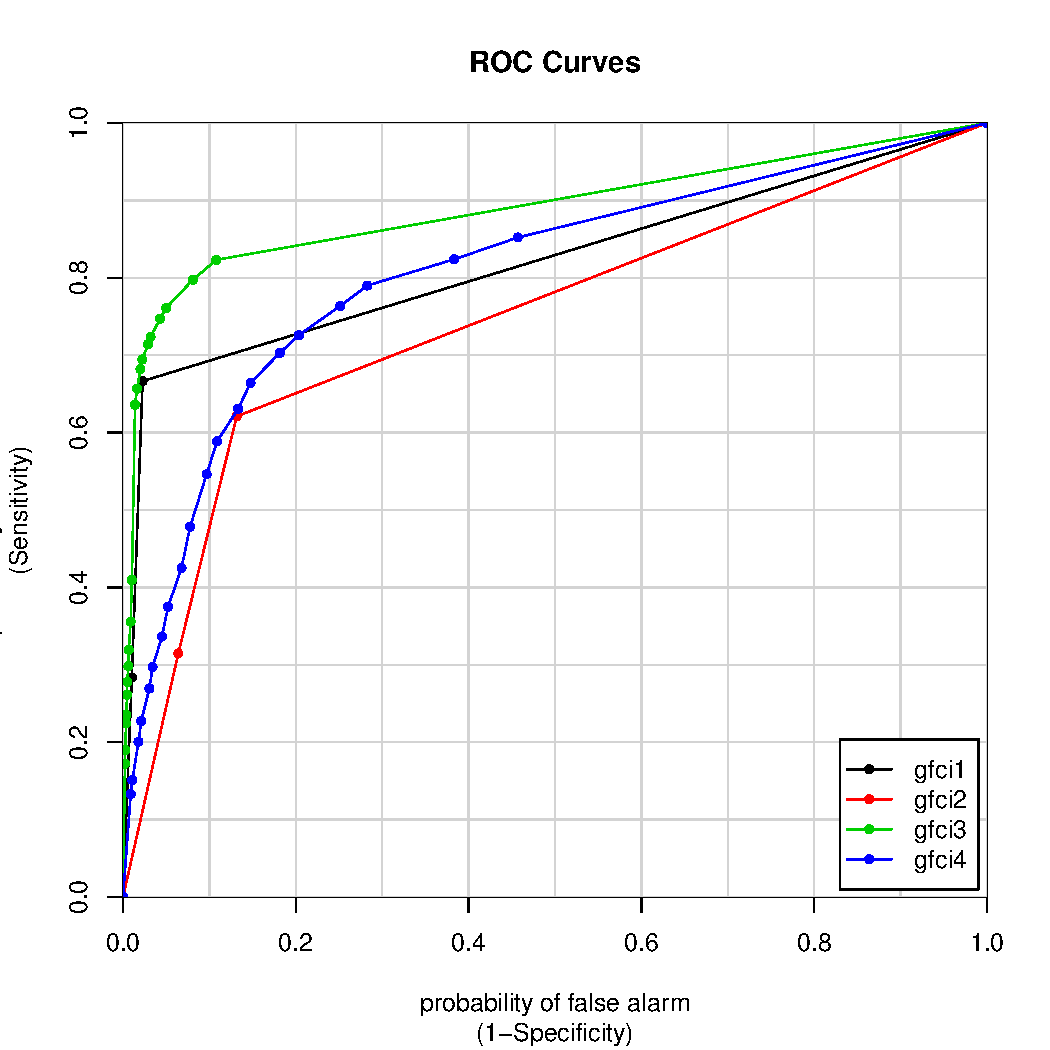
\includegraphics[width=\textwidth]{combinedSimCurvesgfcisim}%
        \end{minipage}\hfill
        \begin{minipage}{0.4\textwidth}
            \centering
            \renewcommand{\arraystretch}{1}
            \setlength{\tabcolsep}{5pt}
            \begin{tabular}{|c|c|c|}
                \multicolumn{3}{c}{\large{\textbf{Legend}}}\\
                \hline
                       & Prior & Bootstrapping\\\
                 GFCI1 & \cmark & \xmark\\
                 GFCI2 & \xmark & \xmark\\
                 GFCI3 & \cmark & \cmark \\
                 GFCI4 & \xmark & \cmark\\
                 \hline
            \end{tabular}
        \end{minipage}
        
    \centering   
    \renewcommand{\arraystretch}{2}
    \setlength{\tabcolsep}{7pt}
    \rowcolors{2}{blue!10}{blue!15}
    \makebox[\textwidth][c]{\begin{tabular}{|c|c|c|c|c|}
        % \multicolumn{5}{c}{\large{\textbf{Non-deterministic JCI-GFCI: Area under ROC curve}}}\\
        \hline
                 & GFCI1 & GFCI2 & GFCI3 & GFCI4\\ \hline
        -1 vs. 1 & 0.8217 & 0.7455 & 0.8894 & 0.8083\\ \hline
    \end{tabular}}
    \caption{ROC curves (top) and Area under ROC curves (bottom) resulting from running GFCI on simulated data. These simulated datasets contained 500 datapoints, 11 system variables and 8 intervention variables. Bootstrapping occurred by running the same algorithm on random subsets of data 10 times and averaging the results. \label{fig:simgraphgfci}}
\end{figure}

\newpage % added for layout
The table in Figure \ref{fig:simgraphgfci} shows that there is a significant increase in area under the ROC curve when GFCI is bootstrapped and prior knowledge is added. This difference is visually illustrated in the graph in Figure \ref{fig:simgraphgfci}, it shows that GFCI3 has the largest area under the curve as well as its value being higher at every point. Moreover, the graph in Figure \ref{fig:simgraphgfci} shows that the application of bootstrapping smooths out the curves for the method. 

\begin{figure}[!ht]
    \centering
    % \large{\textbf{Non-deterministic JCI-FGES run on Simulated Data}}\\
        \centering
        \begin{minipage}{0.6\textwidth}
            \centering
            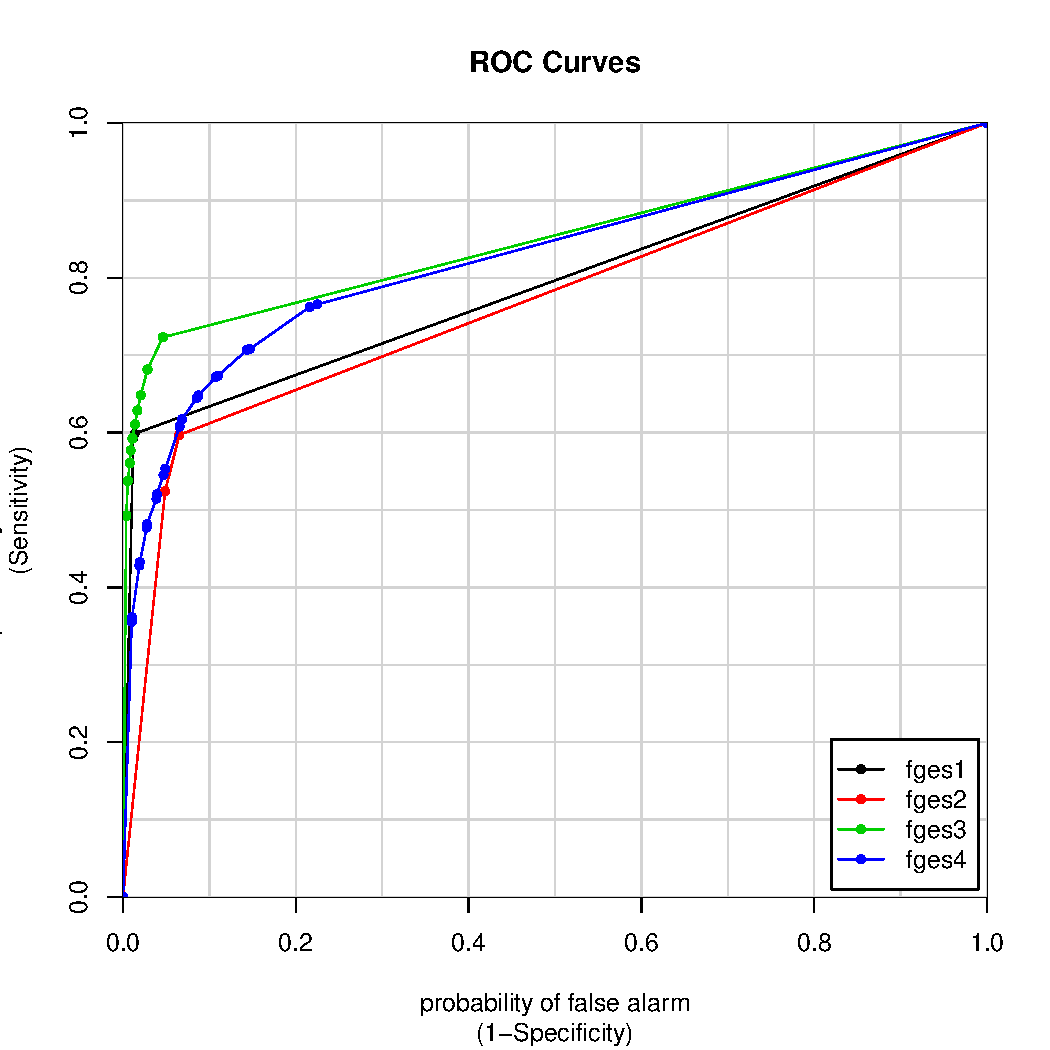
\includegraphics[width=\textwidth]{combinedSimCurvesfgessim}%
        \end{minipage}\hfill
        \begin{minipage}{0.4\textwidth}
            \centering
            \renewcommand{\arraystretch}{1}
            \setlength{\tabcolsep}{5pt}
            \begin{tabular}{|c|c|c|}
                \multicolumn{3}{c}{\large{\textbf{Legend}}}\\
                \hline
                       & Prior & Bootstrapping\\\
                 FGES1 & \cmark & \xmark\\
                 FGES2 & \xmark & \xmark\\
                 FGES3 & \cmark & \cmark \\
                 FGES4 & \xmark & \cmark\\
                 \hline
            \end{tabular}
        \end{minipage}
    \centering   
    \renewcommand{\arraystretch}{2}
    \setlength{\tabcolsep}{7pt}
    \rowcolors{2}{blue!10}{blue!15}
    \makebox[\textwidth][c]{\begin{tabular}{|c|c|c|c|c|}
        % \multicolumn{5}{c}{\large{\textbf{Non-deterministic JCI-FGES: Area under ROC curve}}}\\
        \hline
                 & FGES1 & FGES2 & FGES3 & FGES4\\ \hline
        -1 vs. 1 &0.7930 & 0.7684 & 0.8503 & 0.8260\\ \hline
    \end{tabular}}
    \caption{ROC curves (top) and Area under ROC curves (bottom) resulting from running FGES on simulated data. These simulated datasets contained 500 datapoints, 11 system variables and 8 intervention variables. Bootstrapping occured by running the same algorithm on random subsets of data 10 times and averaging the results.\label{fig:simgraphfges}}
\end{figure}

The table in Figure \ref{fig:simgraphfges} shows that applying JCI to FGES produces similar results to applying JCI to GFCI. Adding the prior knowledge from JCI seems to increase the area under the ROC curve significantly compared to the baseline version for FGES. Looking at the graph in Figure \ref{fig:simgraphfges} and the graph in Figure \ref{fig:obssimgraphfges} demonstrates that bootstrapping combined with prior knowledge has a positive effect on the performance of FGES as well as smoothing out its ROC curve. 


\subsection{Real-world data}

The real-world biological dataset that the non-deterministic JCI framework is applied to, is a dataset first published in a paper by Sachs et al. \cite{sachs2005causal}. Since its publication, the dataset published in this paper has been used in many different papers. The wide use of this dataset allows this paper to be used as a benchmark for the performance of the non-deterministic JCI framework. Its performance can then be compared to that of other research. The system which can be modelled from the dataset provided in the paper, has a generally accepted model. In figure \ref{fig:sachs}, the previously mentioned model can be seen. The system is also sufficiently complex to properly examine the ability of the non-deterministic JCI framework to model the causal relations in a real-world system.

\begin{figure}[!ht]
    \centering
    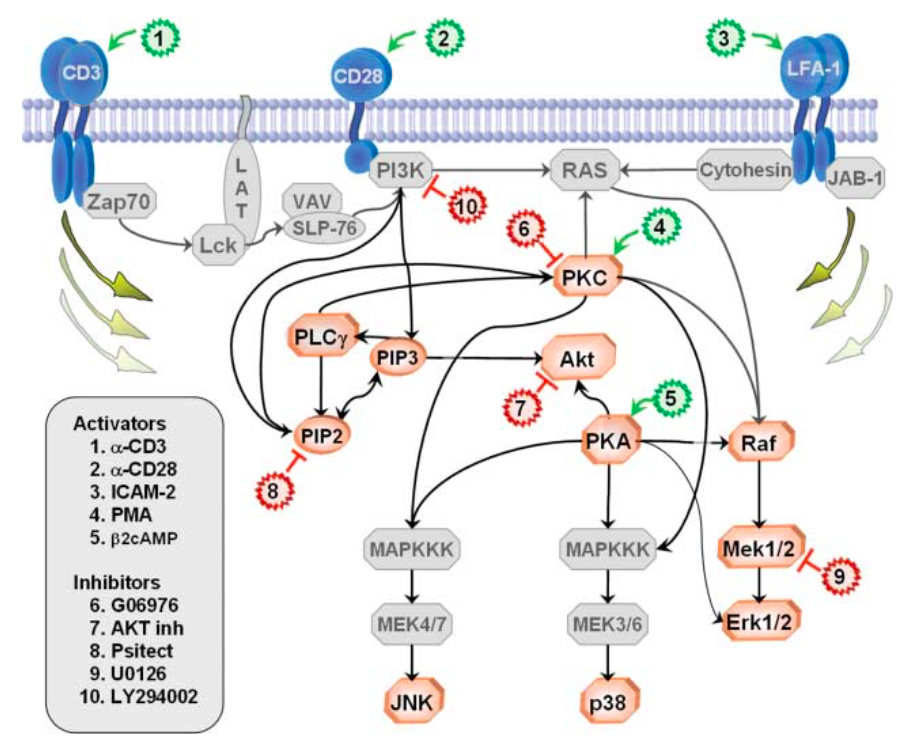
\includegraphics[width=\textwidth]{sachs}
    \caption{Consensus model of protein signalling systems within cells, as illustrated by  Sachs et al. \cite[p.~525]{sachs2005causal} The red spiked nodes represent inhibiting interventions and the green spiked nodes represent activating interventions. The blue nodes are the proteins in the membrane of the cells. The grey cells are latent confounders. }
    \label{fig:sachs}
\end{figure}

In figure \ref{fig:sachs} the consensus model for the real-world dataset is shown. While this model is generally accepted as a likely true model for the causal structures underlying the Sachs dataset, it is not a golden standard. The blue nodes representing the proteins in the cell membrane are not modelled by any of the methods mentioned in this research.

\begin{figure}[!ht]
    \centering
    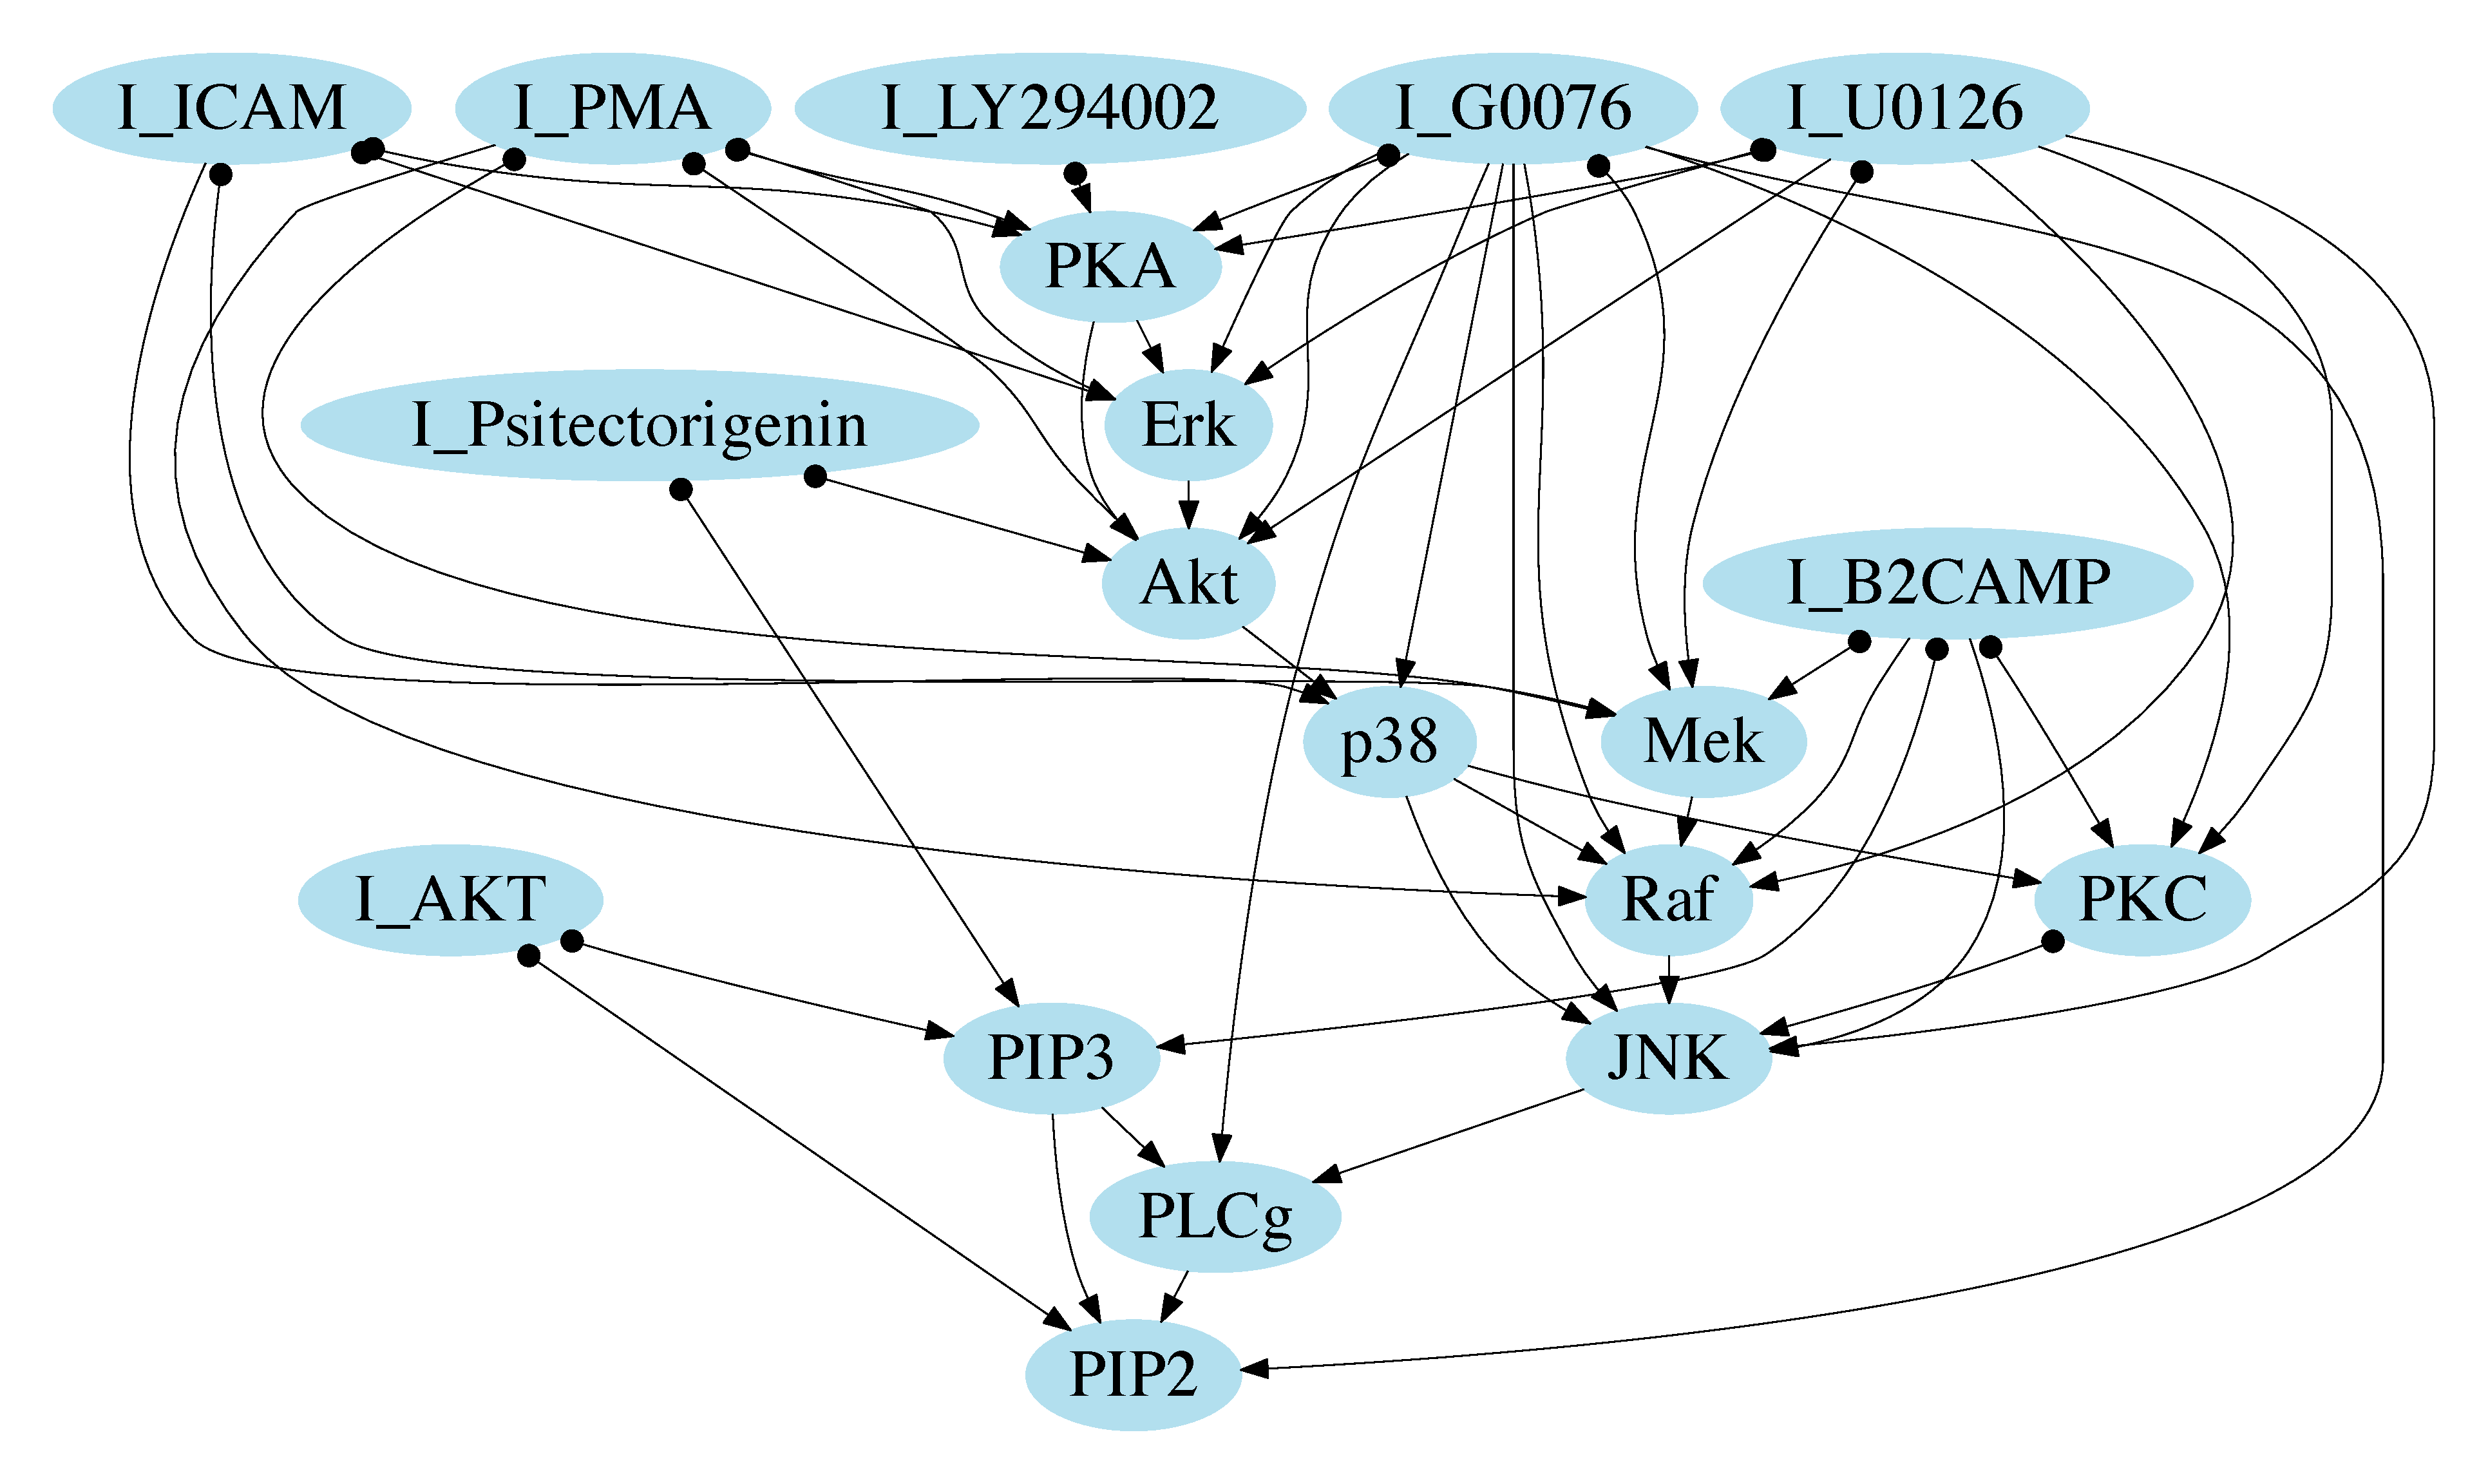
\includegraphics[width=\textwidth]{sachsGraph_bootstrap0_priorTRUEgfci}
    \caption{Results for running GFCI with JCI on Sachs dataset. Shows partial ancestral graph with causal relations inferred from the dataset.}
    \label{fig:sachsGFCIpag}
\end{figure}
\begin{figure}[!ht]
    \centering
    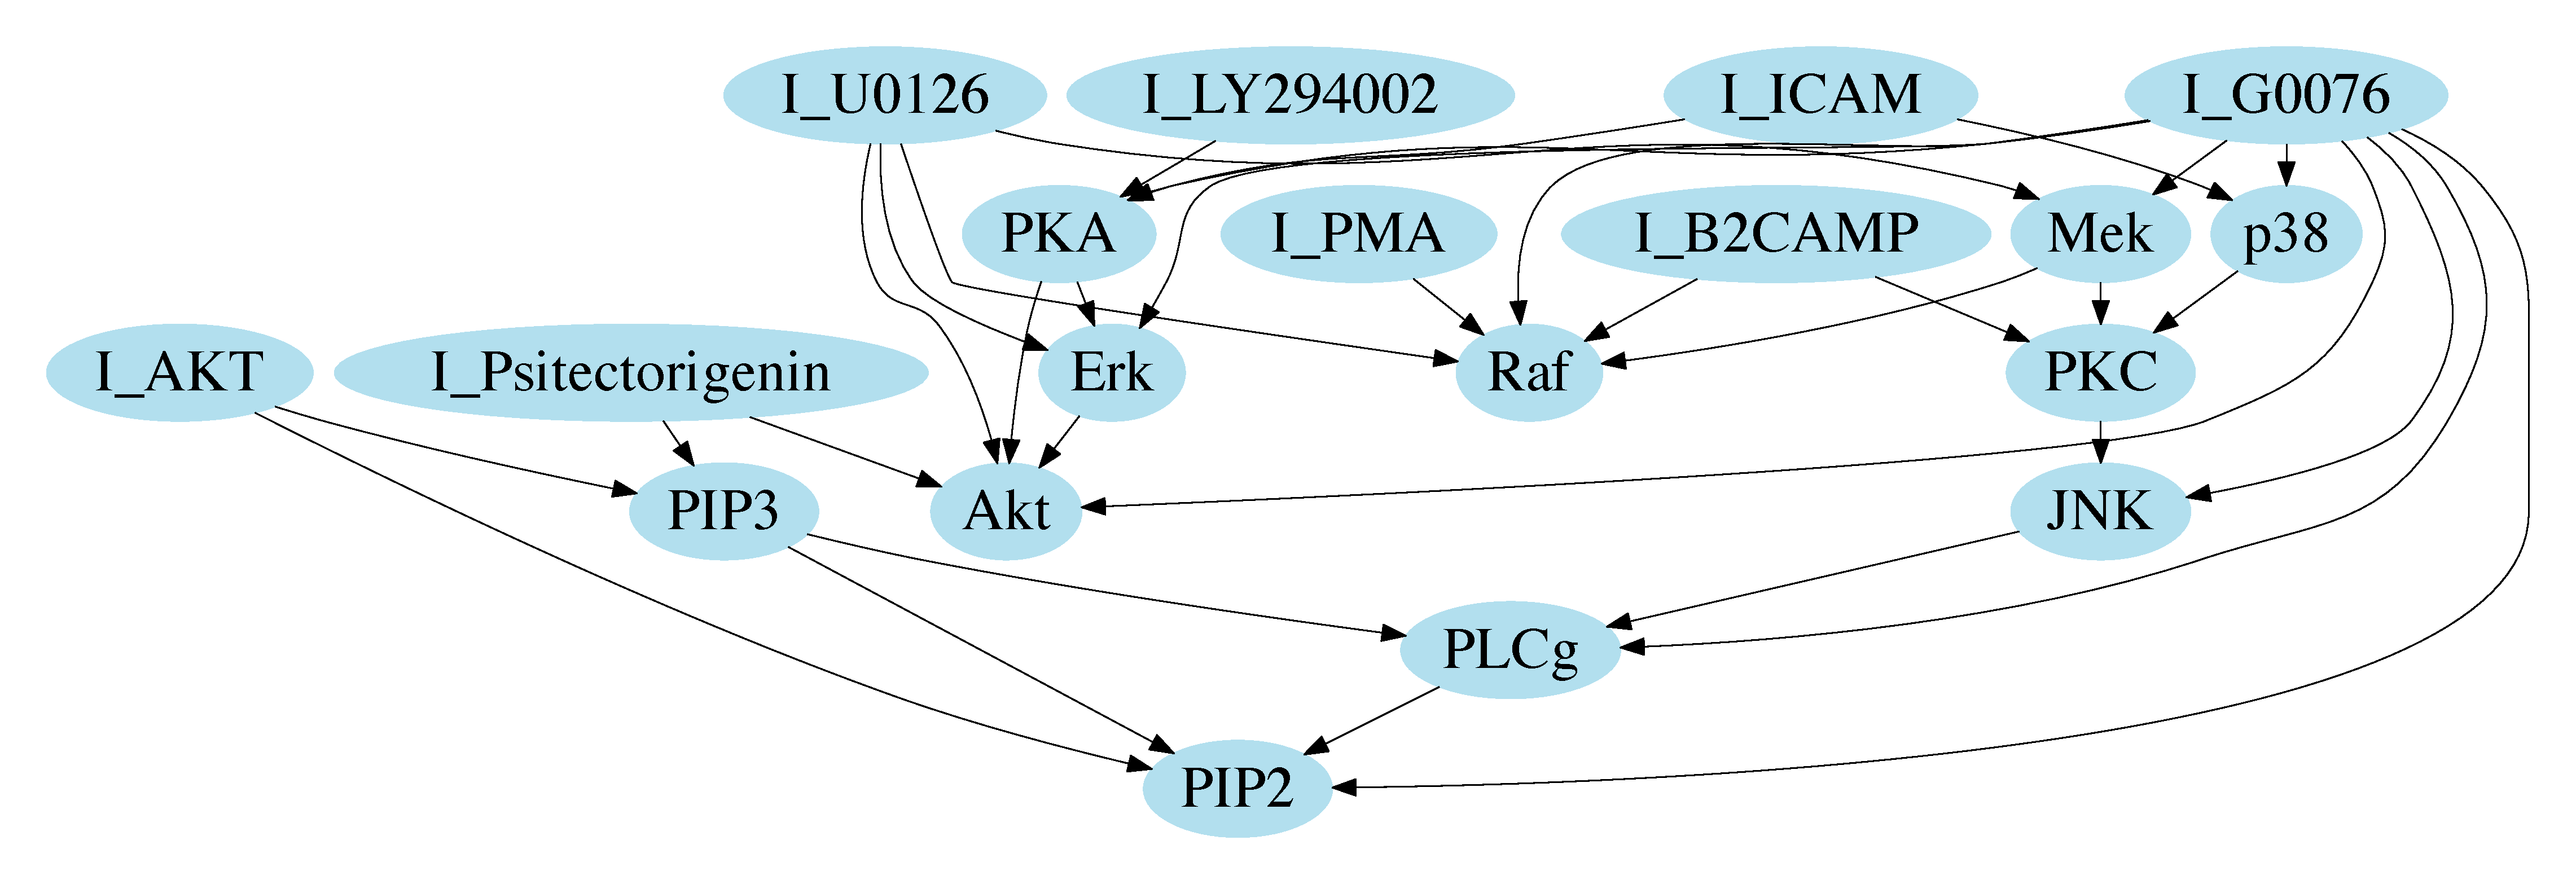
\includegraphics[width=\textwidth]{sachsGraph_bootstrap0_priorTRUEfges}
    \caption{Results for running FGES with JCI on Sachs dataset. Shows partial ancestral graph with causal relations inferred from the dataset.}
    \label{fig:sachsFGESpag}
\end{figure}

When applying GFCI in combination with the JCI framework, a number of relations are found. The prior knowledge which was added prevents the algorithms from making any connections to the intervention variables. The graph illustrating the causal relations found by both methods without prior knowledge from JCI can be found in the appendix. Neither GFCI nor FGES can find a significant number of relations without JCI. Both methods were run on the observational dataset, as neither method can use multiple datasets without JCI. This resulted in GFCI and FGES finding around six relations. Taking into account these baseline measurements, the methods with JCI perform better than those same methods do without JCI.

It is hard to compare these results to methods used outside of this research since the results are not given the same form as for example ACI \cite{aci}, which returns an ancestral structure. Therefore, both Figure \ref{fig:sachsGFCIpag} and Figure \ref{fig:sachsFGESpag} were converted to an ancestral structure. These converted graphs can be found in figure \ref{fig:ACIvsGFCIpriorTRUE} and \ref{fig:ACIvsFGESpriorTRUE}. 


\begin{figure}[!ht]
    \centering
    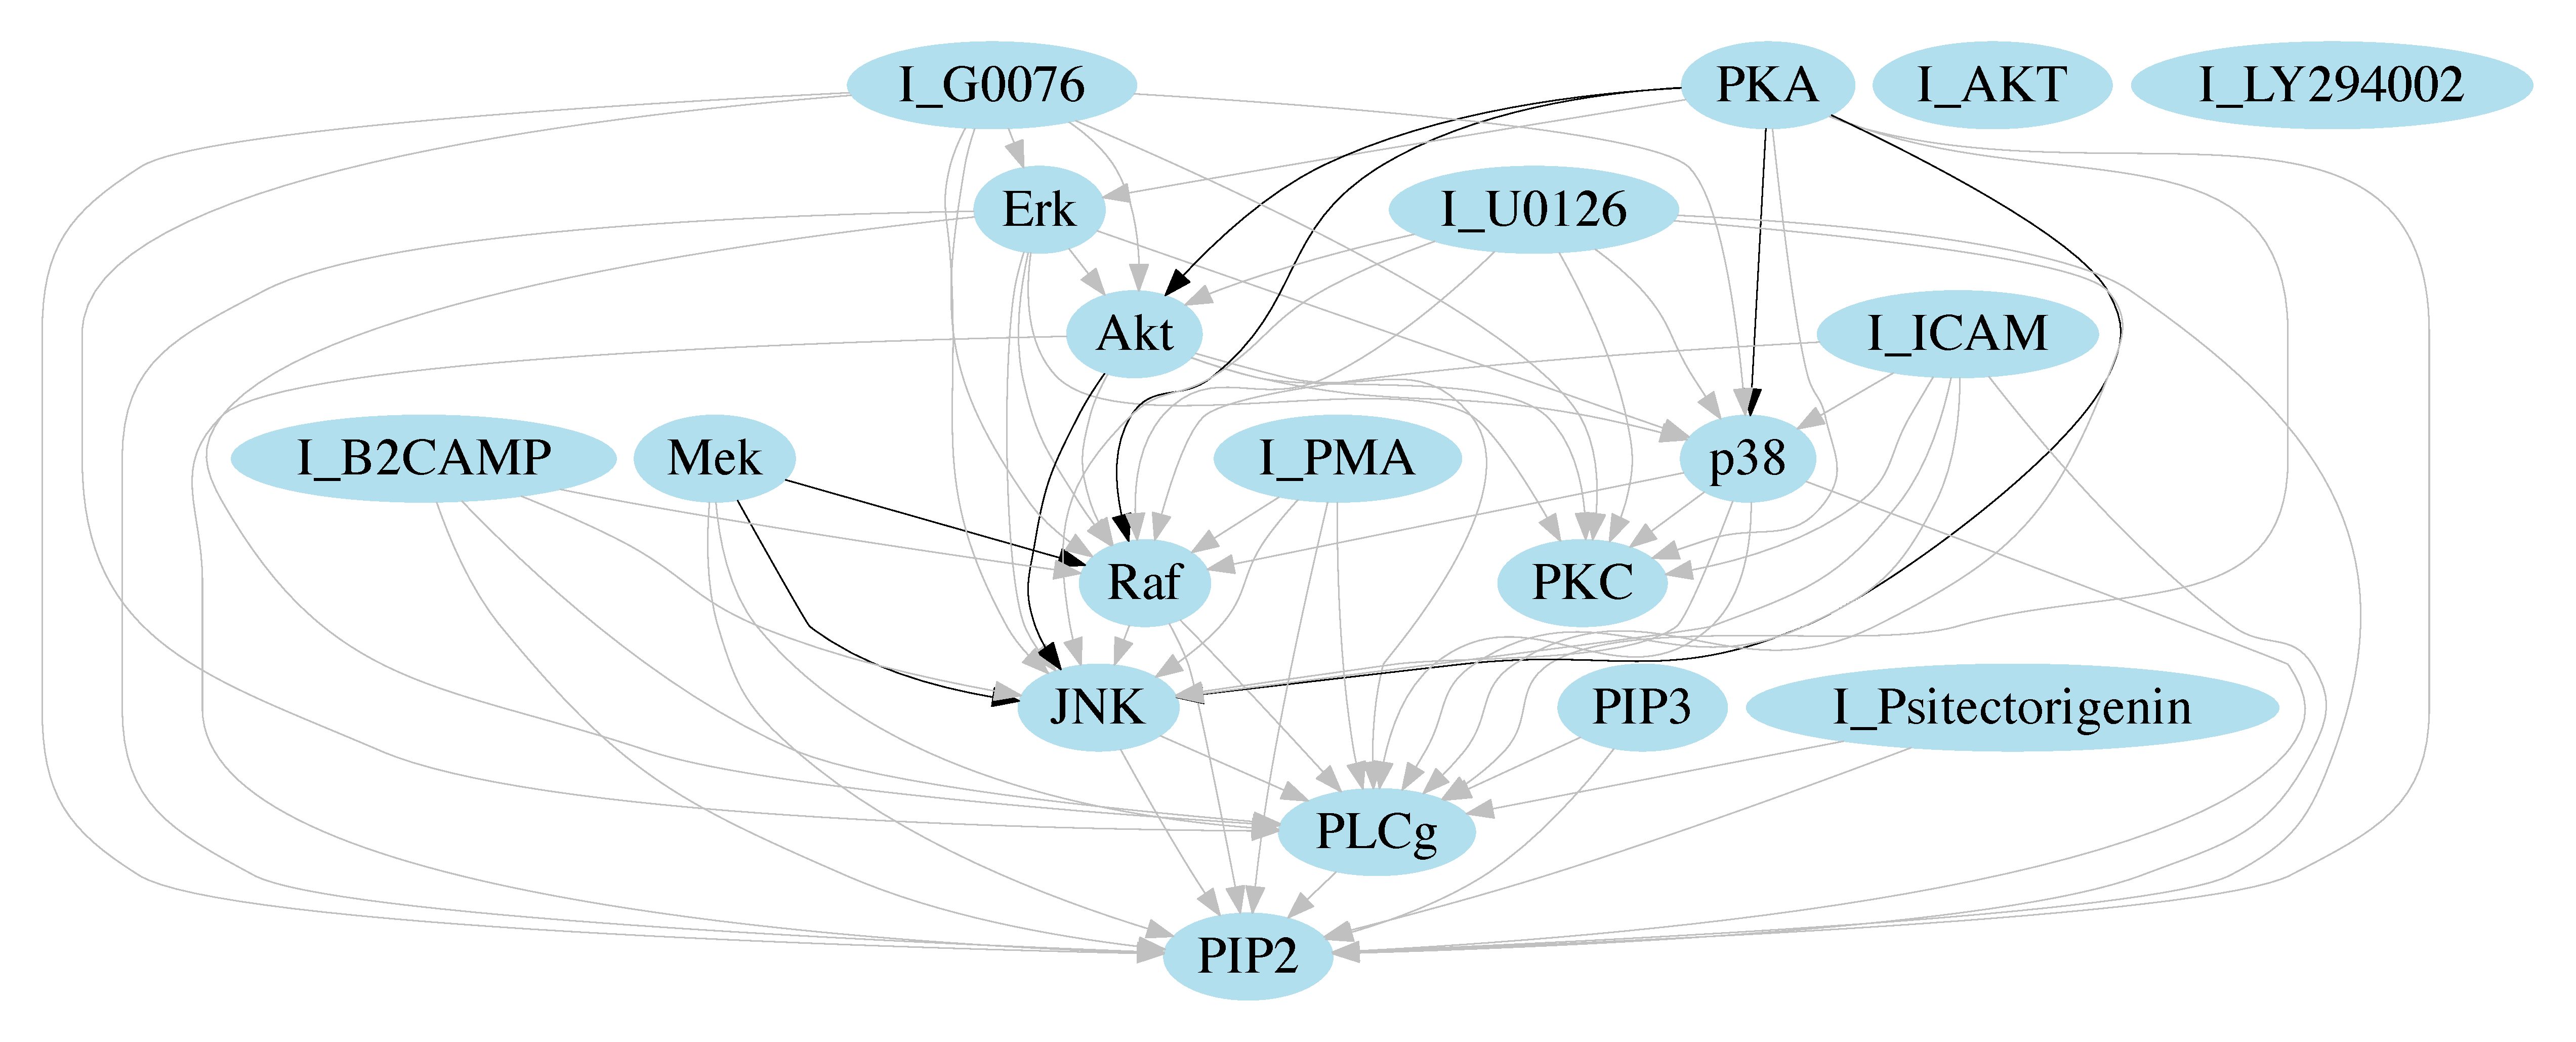
\includegraphics[width=\textwidth]{ACIvsGFCIpriorTRUE}
    \caption{Grey lines are causal connections only found by GFCI, black lines are causal connections found by both ACI and GFCI.}
    \label{fig:ACIvsGFCIpriorTRUE}
\end{figure}
\begin{figure}[!ht]
    \centering
    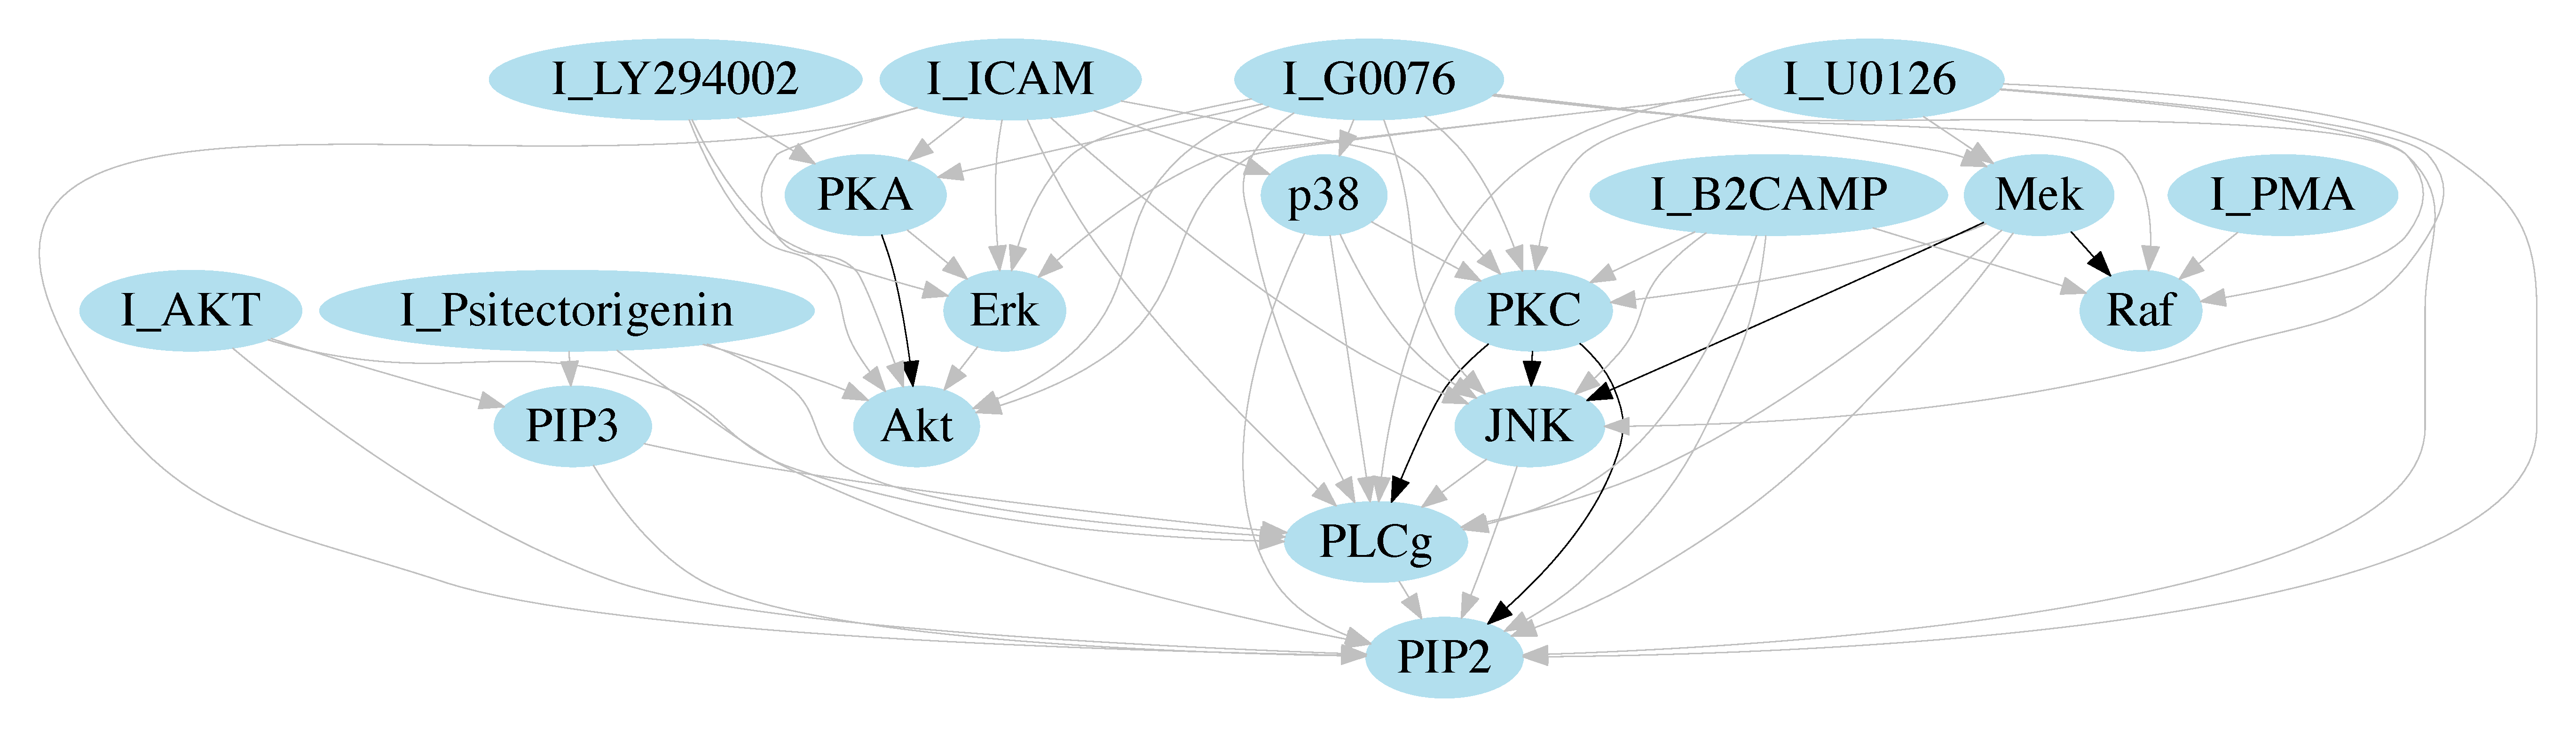
\includegraphics[width=\textwidth]{ACIvsFGESpriorTRUE}
    \caption{Grey lines are causal connections only found by FGES, black lines are causal connections found by both ACI and FGES.}
    \label{fig:ACIvsFGESpriorTRUE}
\end{figure}

When comparing these ancestral structures to each other, it is important to note that a limited amount of methods are able to learn the intervention targets. Without the JCI framework, ACI cannot learn the intervention targets. In the figures \ref{fig:ACIvsGFCIpriorTRUE} and \ref{fig:ACIvsFGESpriorTRUE}, it is visible that the overlap in relations found between ACI and the methods in this research is small.

\section{Conclusion \& Discussion}

% \Sara{This is definitely too long and with too much repetition. You just need to say something like one or two paragraphs per research questions and leave out details, for example which packages you used for the implementation.}

% reiterate what the questions are and why they need to be asked
The research started out by posing the first research question, which is ``How does Joint Causal Inference perform on real-world datasets?'' In seeking to answer this question, some problems arose, namely the scalability of JCI. JCI is limited to a small number of variables, as it does not scale up well enough. Moreover, the deterministic relations caused by JCI are problematic, since it limits the amount of choice in methods to be used. Therefore, the second research question was posed: ``How can one implement a simplified version of Joint Causal Inference that scales up to the number of variables in a real-world dataset?''. This second research question must be answered in order to be able to answer the first research question.

% how did we implement jci: dataset
By finding and removing deterministic relations from the intervention variables in the dataset and adding prior knowledge to methods performing causal inference, a non-deterministic version of JCI was implemented. The removal of deterministic relations in the real-world dataset was achieved by executing the operations as described in the non-deterministic JCI section. This enabled a non-deterministic configuration of the intervention variables in the real-world Sachs dataset. 

% how did we implement jci: prior knowledge
The addition of prior knowledge to methods performing causal inference was achieved making use of the rcausal package \cite{r-wrapper}. With this prior knowledge one of the JCI assumptions could be implemented into these methods. The implementation of prior knowledge and removal of deterministic relations, constitute a simplified version of the JCI framework. By implementing these two criteria, the second research question has been answered. With this method it is possible to implement a simplified version of JCI.

% first question: simdata impact
After successfully answering the second research question, the first question can be examined. The application of JCI on simulated data, shows that the JCI framework improves the performance of methods when measured with ROC curves. Using JCI and bootstrapping can increase the area under the ROC curve of a method by as much as $0.27$. Furthermore, looking at the tables for both GFCI and FGES in figures \ref{fig:obssimgraphgfci}, \ref{fig:obssimgraphfges}, \ref{fig:simgraphgfci} and \ref{fig:simgraphfges} shows that both methods benefit from the application of JCI. It also shows that GFCI has better performance than FGES. Consequently, GFCI is a more favourable method by this metric. Moreover, GFCI also accounts for latent confounders while FGES does not, which allows for a closer approximation of the true model as real-world data often contains unmeasured and unknown variables. 

% first question: sachs results
Examining the results of the application of GFCI-JCI on the Sachs dataset shows that 16 found relations between system variables overlap with causal relations found by other methods. The overlap with the consensus model is significantly smaller at 7 common relations. Without an expert in protein signalling systems these results are difficult to interpret. It is, however, safe to say that the application of the JCI framework improved the performance of both methods tested in this research. Neither GFCI nor FGES was able to find a significant number of causal relations from the observational dataset without JCI. The full comparison between GFCI, FGES and other methods such ACI can be found in Table \ref{tab:comparisonSachs}.

% final remarks/summary
In conclusion, the application of JCI improves the performance of methods on simulated data. When comparing the results of methods with and without JCI on real-world data, it is clear that JCI enables methods to infer more causal relations from this data. While the plausibility of the results is hard to interpret without expert knowledge, comparison with other methods shows overlap between causal relations found by methods in this research, and other methods, as well as the consensus model.

\section{Future Work}
With this research a non-deterministic version of JCI has been applied to simulated data, showing that the application increased the performance of two different algorithms. Considering that the application of bootstrapping to these methods further increased the performance, it would be wise to apply bootstrapping to real-world data as well. Due to the small number of data points, this method cannot be applied to the Sachs dataset. Another possible research direction that could improve the accuracy of the methods would be to add more background knowledge to the current implementation. Specifically, better results could be achieved by adding to the background knowledge that no hidden variables can cause both intervention variables and system variables. 

Moreover, an expert in protein signalling networks could be asked to evaluate the results of this research. Having an expert determine the plausibility of the connections made, could give more insight in how well the algorithm is doing and what can be improved. 

Finally, a different method for applying JCI to real-world data can be explored. It might be possible to scale the complete deterministic version of JCI to a number of variables appropriate for real-world data. The possibility of creating a theoretically sound method to combine multiple graphs generated by JCI could be explored.  

\bibliographystyle{abbrv}
\bibliography{ref1} 

\newpage
\appendix
\section{Additional Results}
All of the code used in this research can be found in the github repository at https://github.com/regenworm/aci
\begin{figure}[!ht]
    \centering
    \large{\textbf{GFCI run on Observational Simulated Data}}\\
        \begin{minipage}{0.6\linewidth}
            \centering
            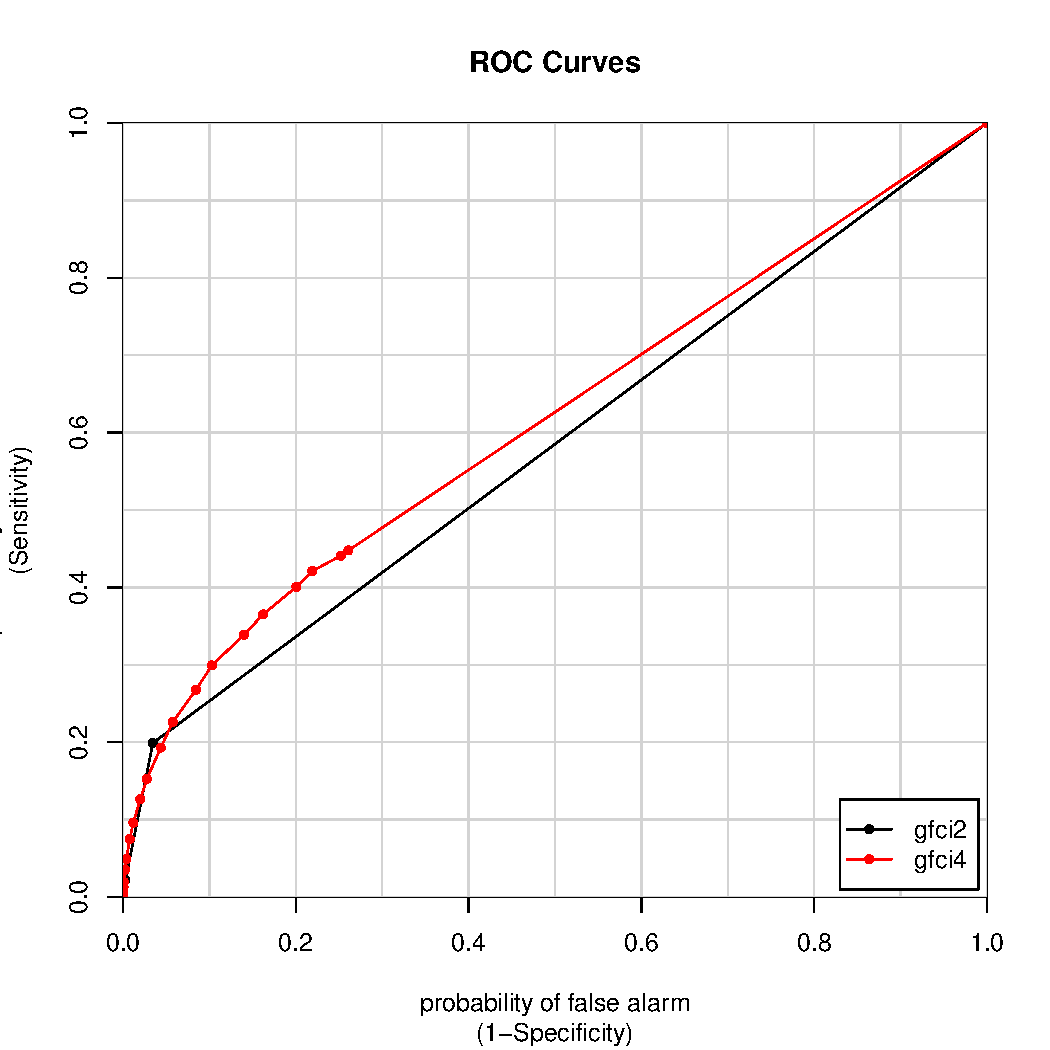
\includegraphics[width=\textwidth]{combinedSimCurvesgfciobsSim}
        \end{minipage}
        \begin{minipage}{0.3\linewidth}
        {\footnotesize
            %\centering
            \renewcommand{\arraystretch}{1}
            \setlength{\tabcolsep}{5pt}
            \begin{tabular}{|r|c|c|}
              \multicolumn{3}{c}{\large{\textbf{Legend}}}\\
                \hline
                       & Prior & Bootstrapping\\\
                 GFCI2 & \xmark & \xmark\\
                 GFCI4 & \xmark & \cmark\\
                 \hline
            \end{tabular}
            }
        \end{minipage}\hfill

    \centering   
    \renewcommand{\arraystretch}{2}
    \setlength{\tabcolsep}{7pt}
    \rowcolors{2}{blue!10}{blue!15}\begin{tabular}{|r|c|c|}
        \multicolumn{3}{c}{\large{\textbf{Area under ROC curve for the different versions of GFCI}}}\\
        \hline
                 & GFCI2 & GFCI4\\ \hline
        -1 vs. 1 & 0.5823 & 0.6153\\ \hline
    \end{tabular}
    \caption{ROC curves (top) and Area under ROC curves (bottom) resulting from running GFCI on only the observational data of a simulated dataset. These simulated datasets contained 500 datapoints, 11 system variables and 8 intervention variables. The intervention variables were ignored as their targets cannot be learned by GFCI without JCI. Bootstrapping occurred by running the same algorithm on random subsets of data 10 times and averaging the results.\label{fig:obssimgraphgfcifull}}

\end{figure}
\begin{figure}[!ht]
    \centering
    \large{\textbf{FGES run on Observational Simulated Data}}\\
        \begin{minipage}{0.6\linewidth}
            \centering
            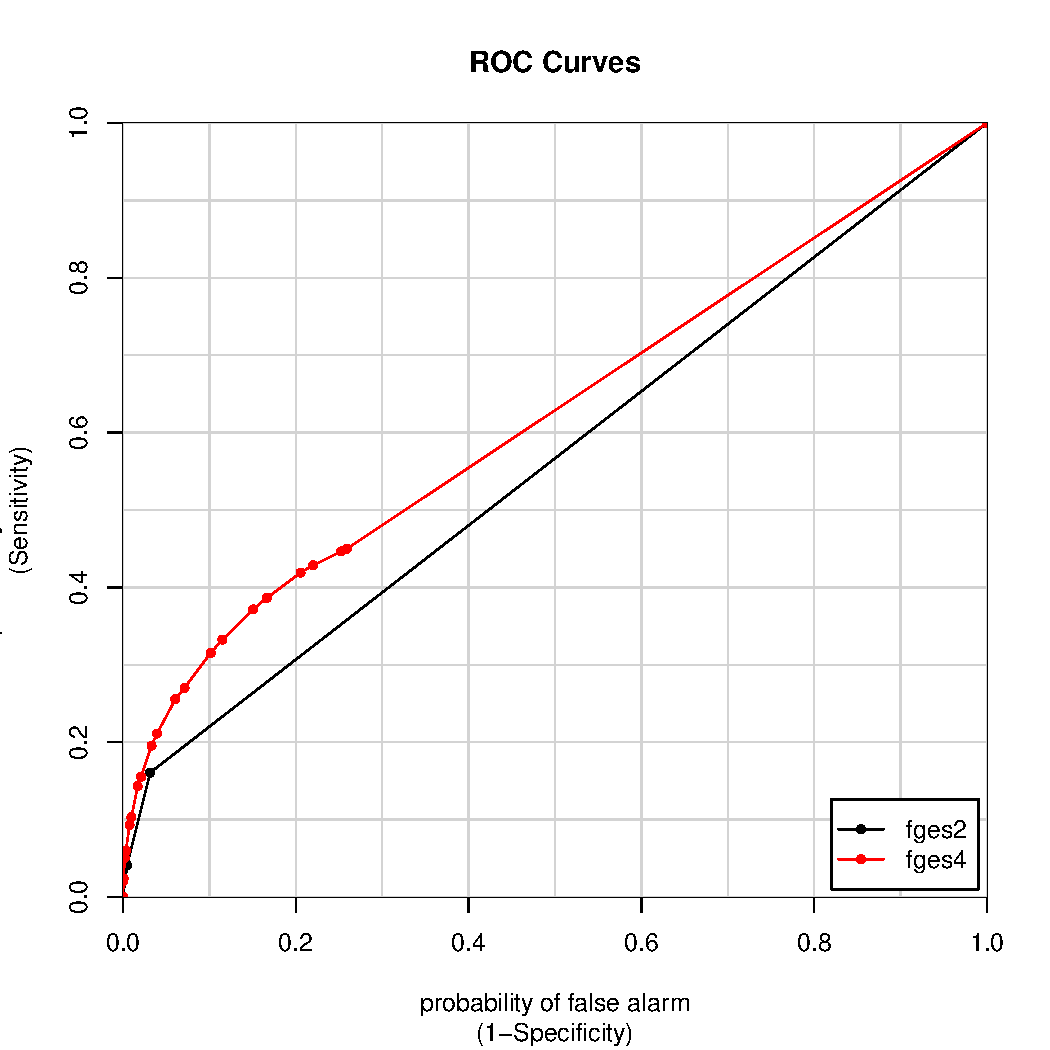
\includegraphics[width=\textwidth]{combinedSimCurvesfgesobsSim}
        \end{minipage}
        \begin{minipage}{0.3\linewidth}
        {\footnotesize
            %\centering
            \renewcommand{\arraystretch}{1}
            \setlength{\tabcolsep}{5pt}
            \begin{tabular}{|r|c|c|}
              \multicolumn{3}{c}{\large{\textbf{Legend}}}\\
                \hline
                       & Prior & Bootstrapping\\\
                 FGES2 & \xmark & \xmark\\
                 FGES4 & \xmark & \cmark\\
                 \hline
            \end{tabular}
            }
        \end{minipage}\hfill

    \centering   
    \renewcommand{\arraystretch}{2}
    \setlength{\tabcolsep}{7pt}
    \rowcolors{2}{blue!10}{blue!15}
    \makebox[\textwidth][c]{\begin{tabular}{|r|c|c|}
        \multicolumn{3}{c}{\large{\textbf{Area under ROC curve for the different versions of FGES}}}\\
        \hline
                 & FGES2 & FGES4\\ \hline
        -1 vs. 1 & 0.5649 & 0.6213\\ \hline
    \end{tabular}}
    \caption{ROC curves (top) and Area under ROC curves (bottom) resulting from running FGES on only the observational data of a simulated dataset. These simulated datasets contained 500 datapoints, 11 system variables and 8 intervention variables. The intervention variables were ignored as their targets cannot be learned by FGES without JCI. Bootstrapping occurred by running the same algorithm on random subsets of data 10 times and averaging the results.\label{fig:obssimgraphfgesfull}}

\end{figure}

\begin{figure}[!ht]
    \centering
    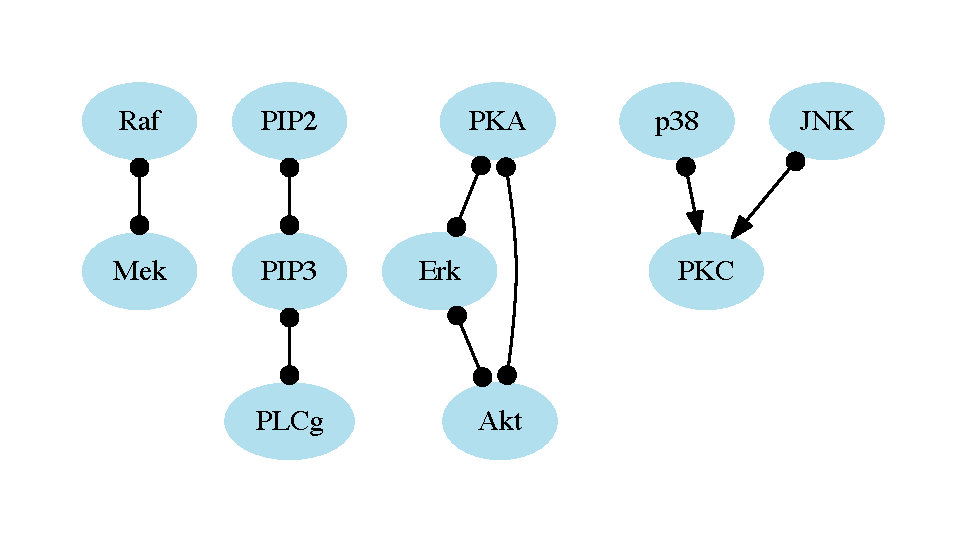
\includegraphics[width=\textwidth]{additional/obsSachsGraph_bootstrap0_priorFALSEgfci}
    \caption{Resulting partial ancestral graph after applying baseline for GFCI to Sachs dataset. In the converted ancestral graph none of the relations remain.\label{fig:obsSachsPagsgfci}}
\end{figure}
\begin{figure}[!ht]
    \centering
    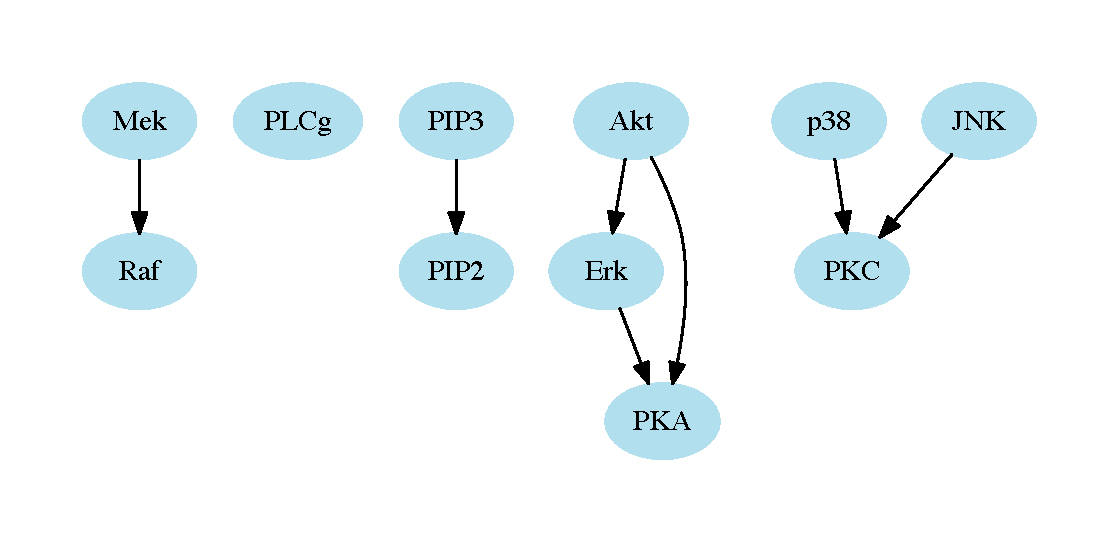
\includegraphics[width=\textwidth]{additional/obsSachsGraph_bootstrap0_priorFALSEfges}
    \caption{Resulting partial ancestral graph after applying baseline for FGES to Sachs dataset. In the converted ancestral graph only the relations to PKC remain. \label{fig:obsSachsPagsfges}}
\end{figure}
\newpage

\begin{figure}[!ht]
    \centering
    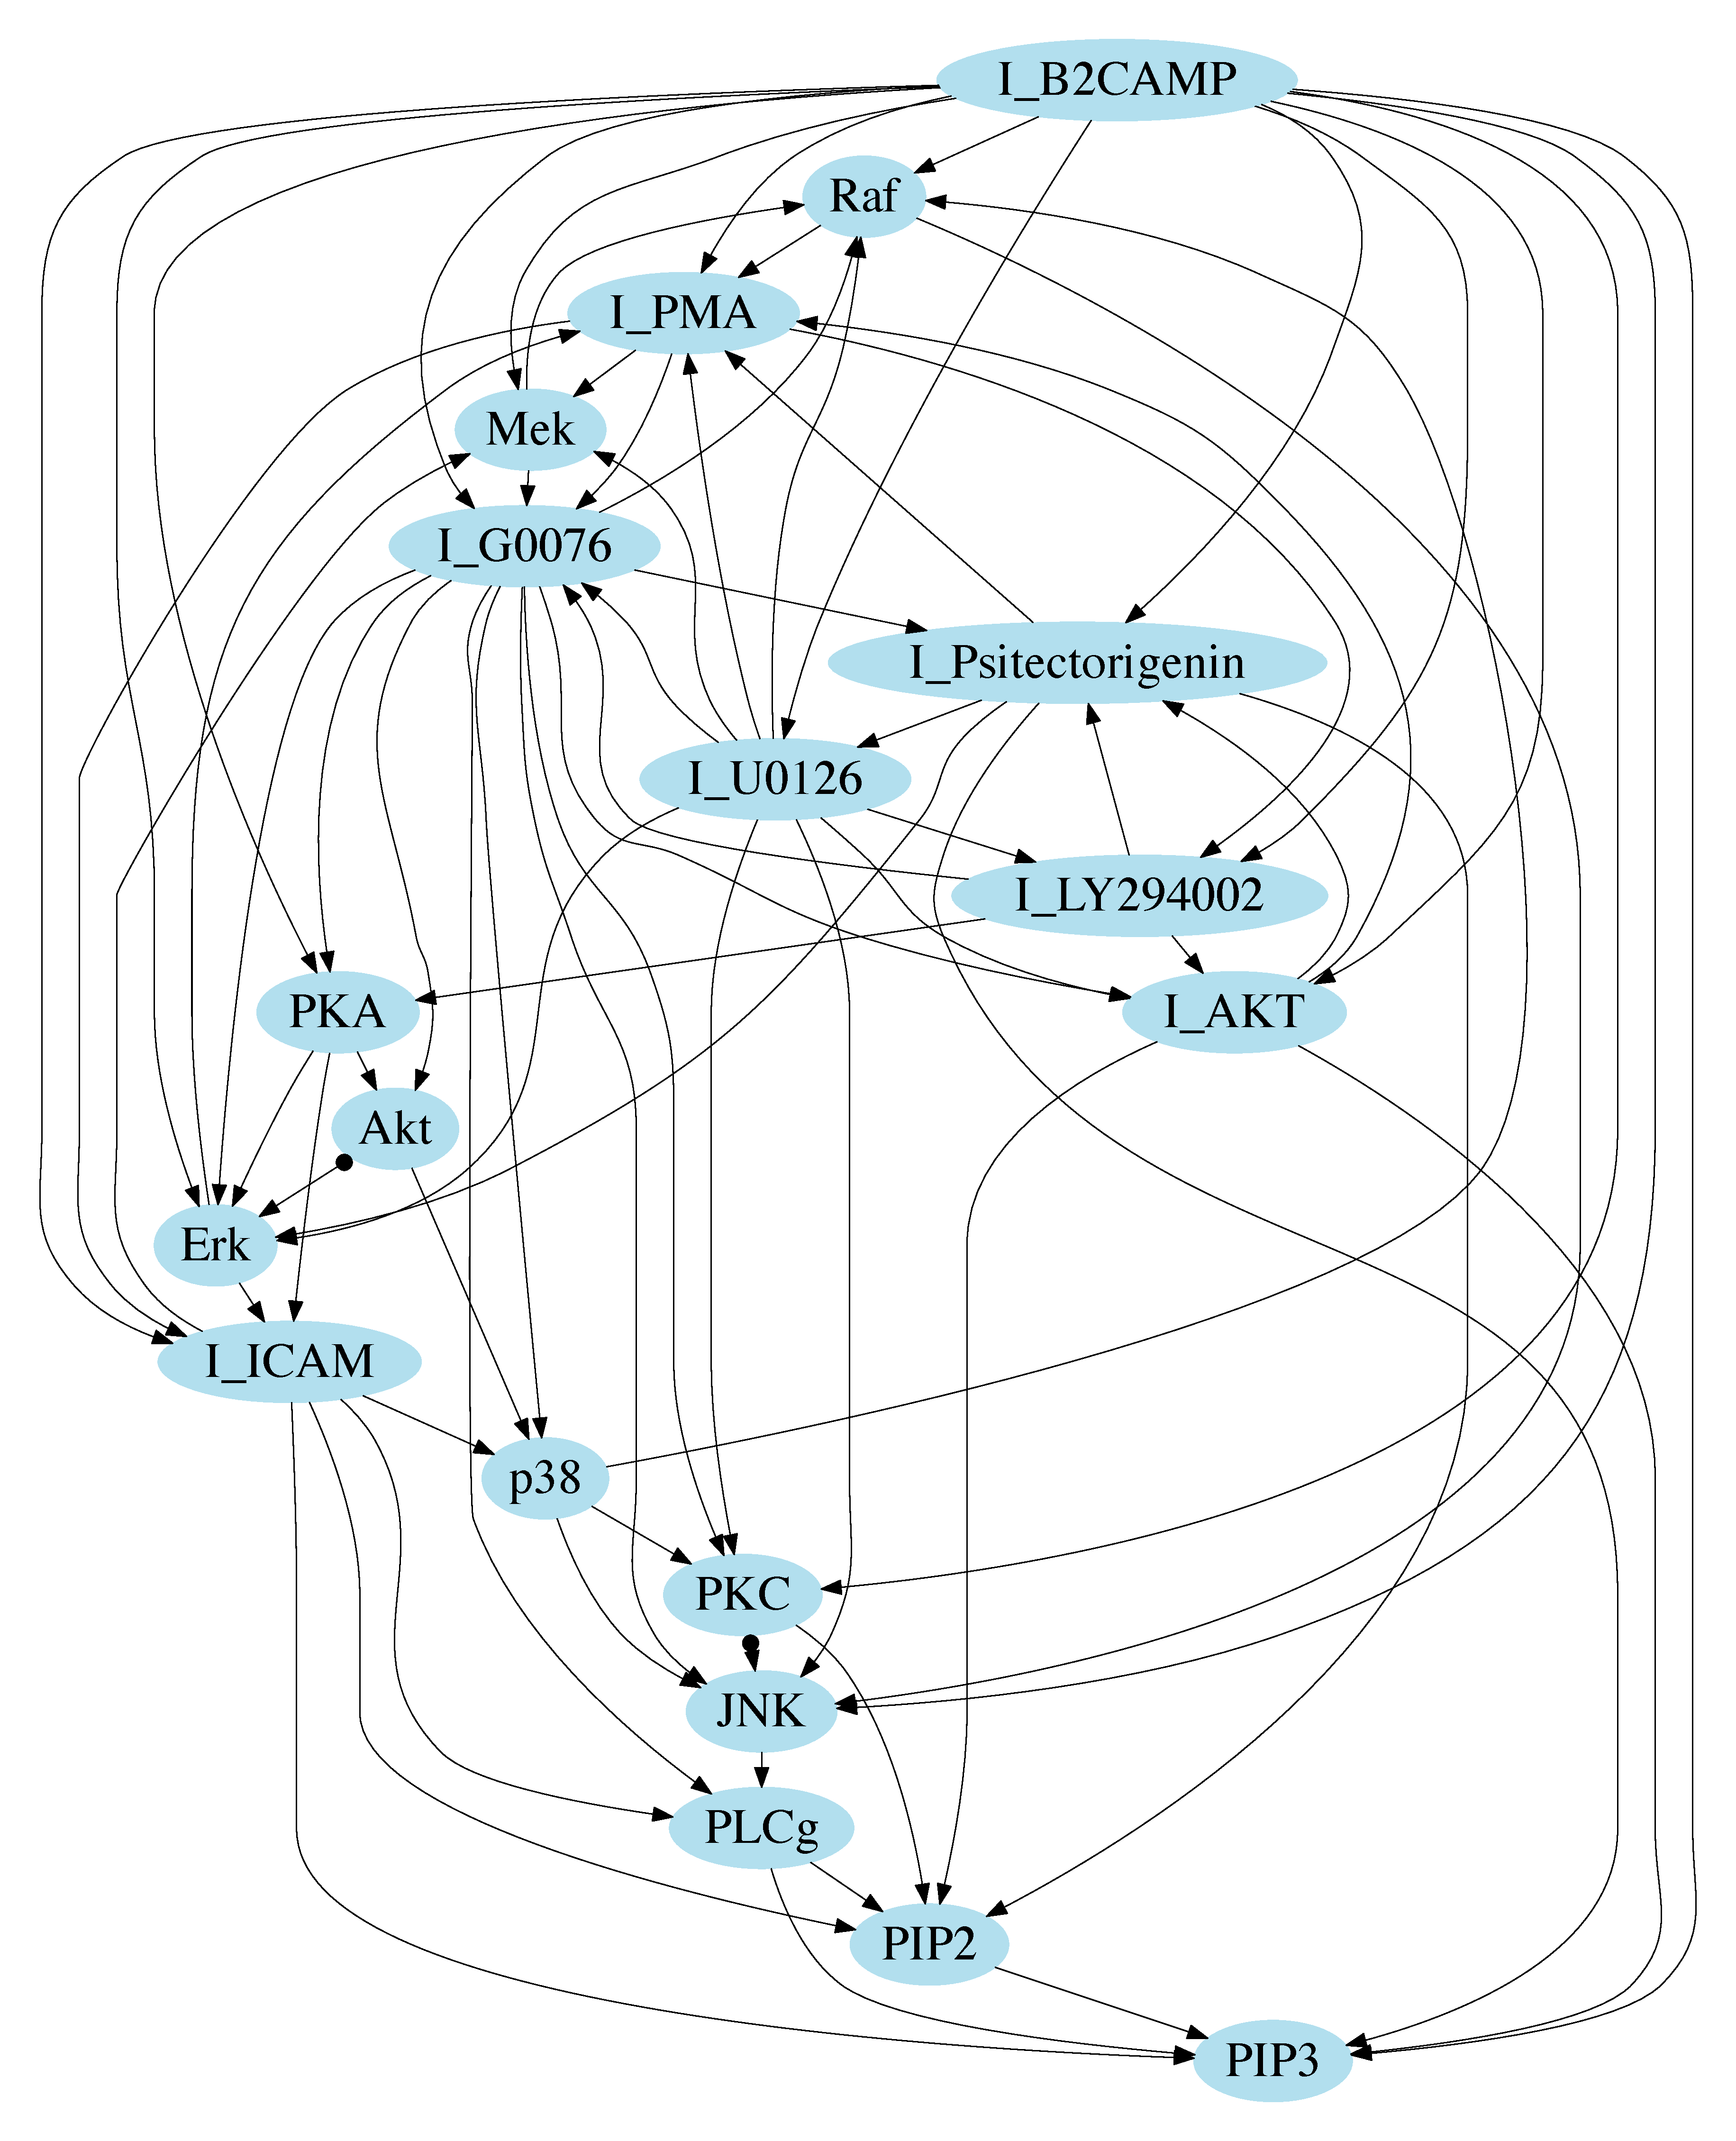
\includegraphics[width=\textwidth]{additional/sachsGraph_bootstrap0_priorFALSEgfci}
    \caption{Resulting partial ancestral graph after applying GFCI to Sachs dataset without a prior. \label{fig:sachspagnopriorgfci}}
\end{figure}
\begin{figure}[!ht]
    \centering
    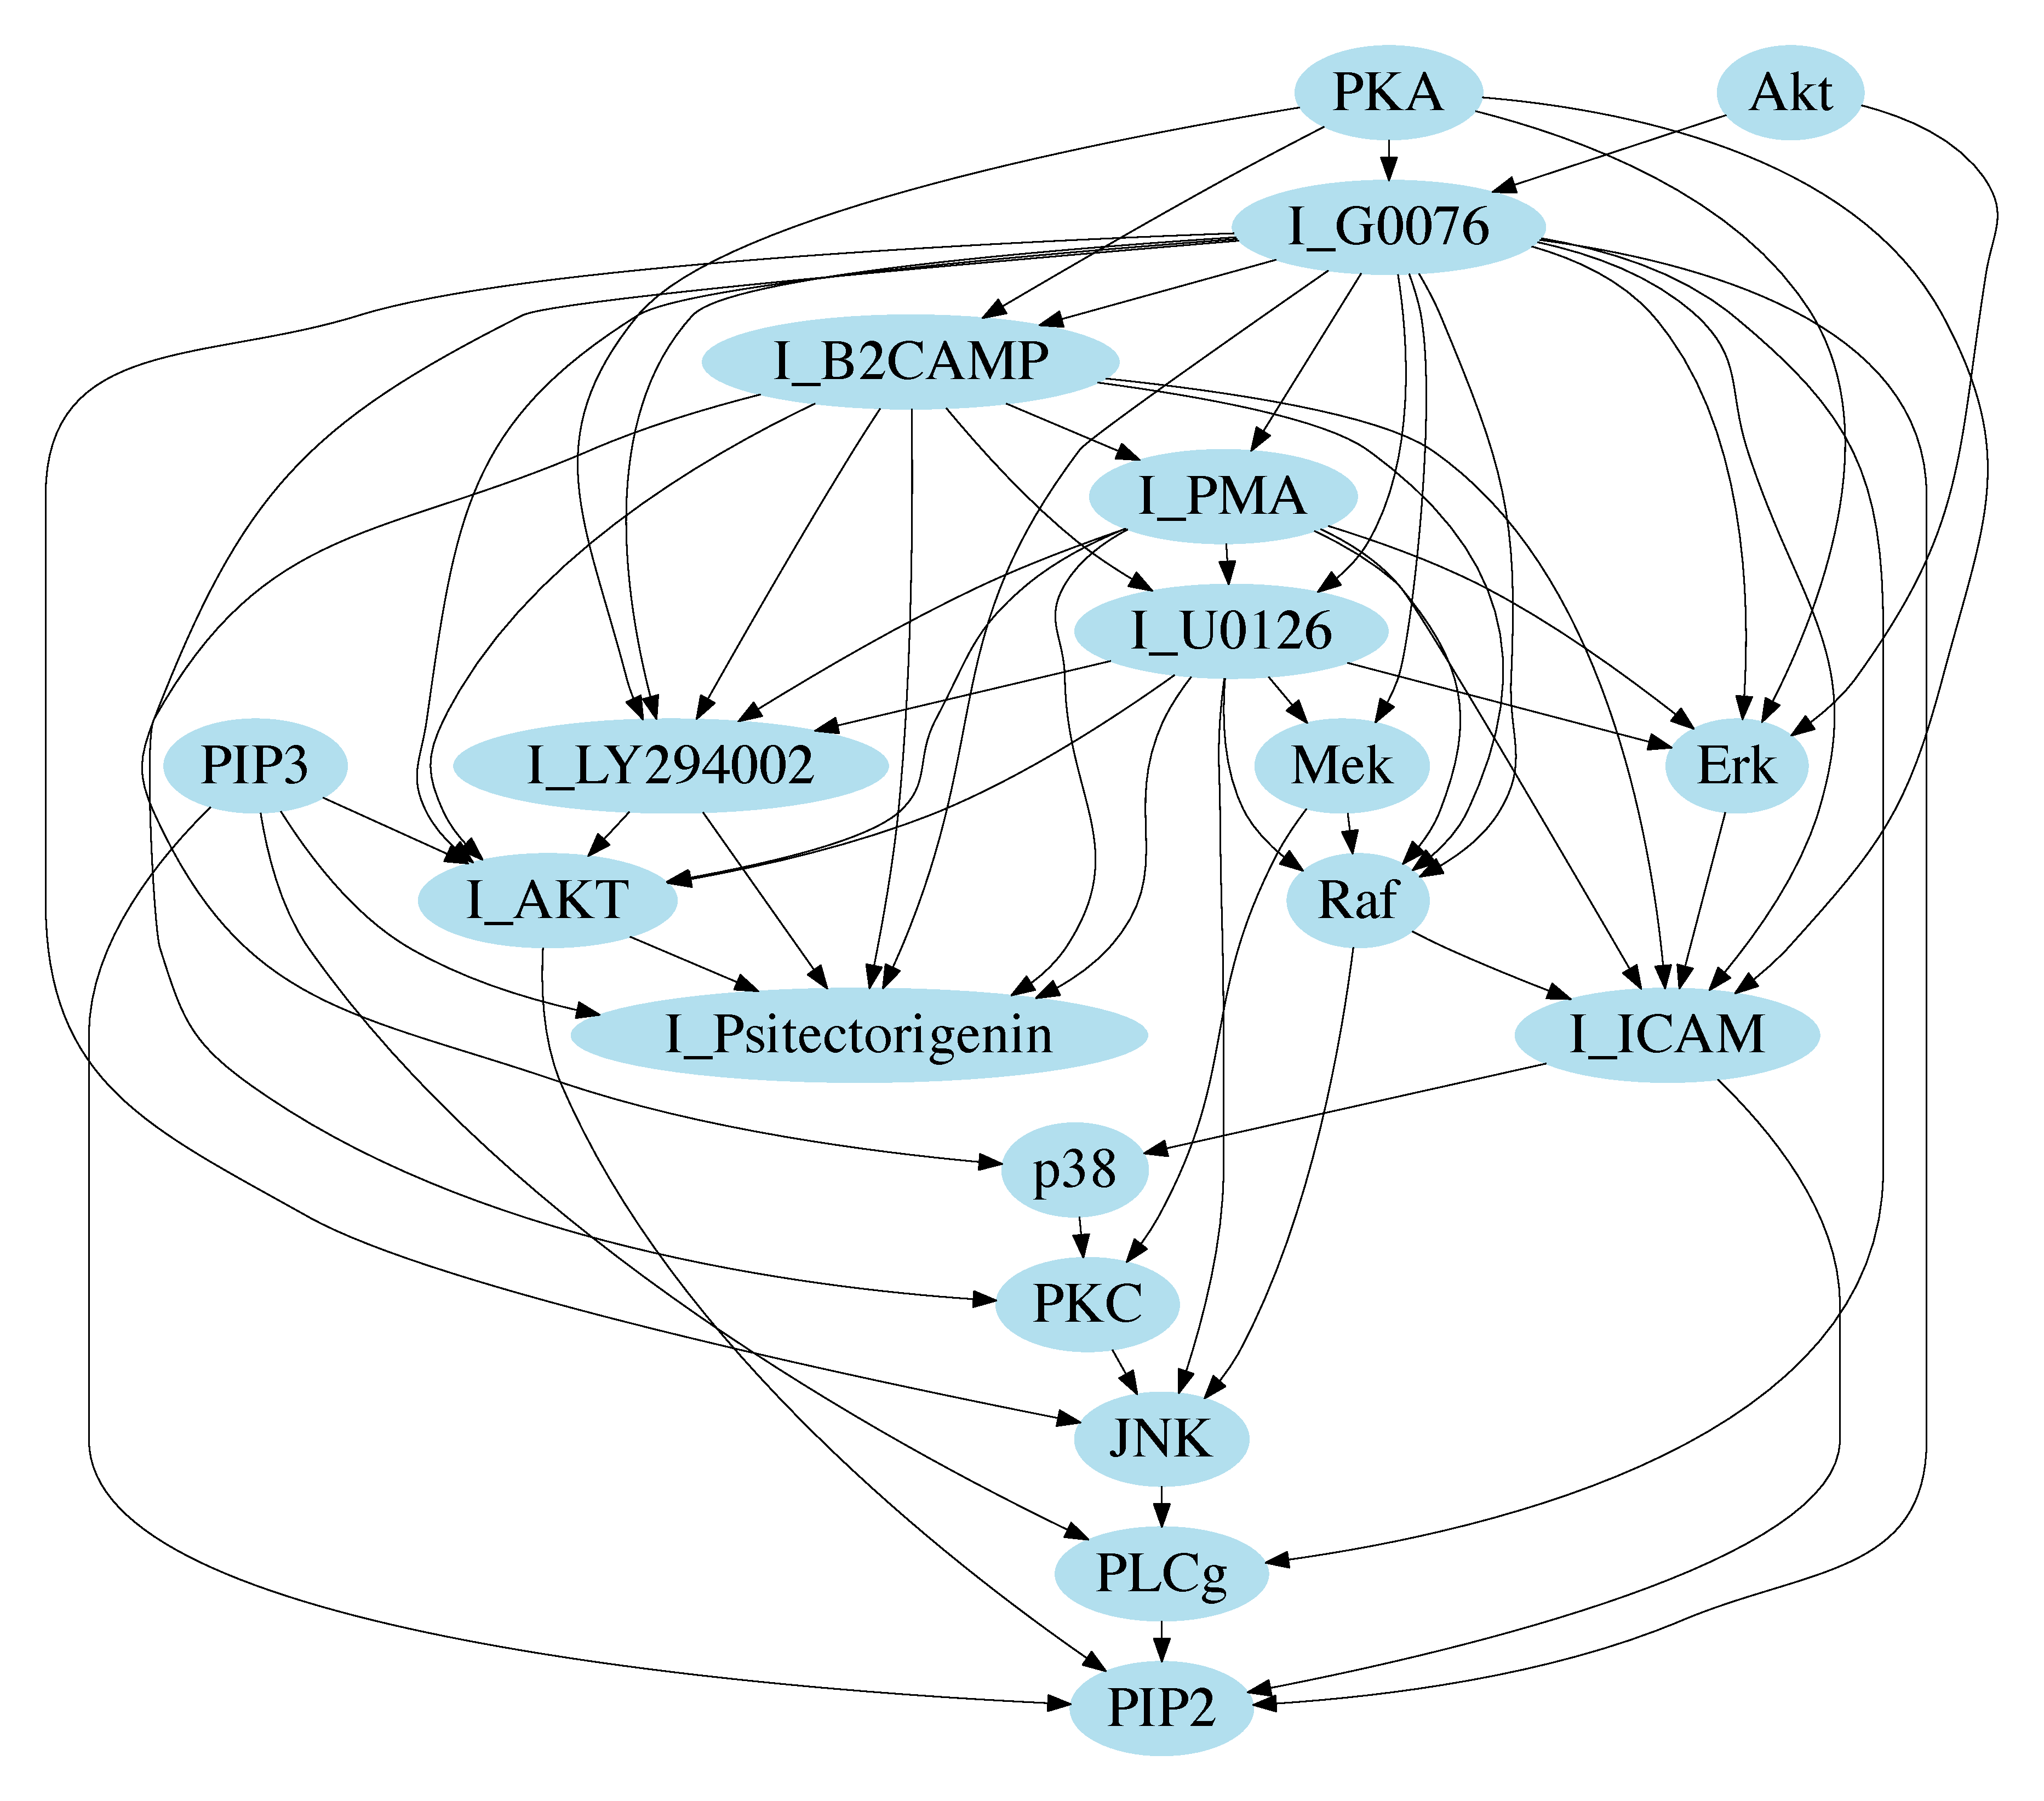
\includegraphics[width=\textwidth]{additional/sachsGraph_bootstrap0_priorFALSEfges}
    \caption{Resulting graph after applying FGES to Sachs dataset without a prior. \label{fig:sachspagnopriorfges}}
\end{figure}

\begin{figure}[!ht]
    \centering
    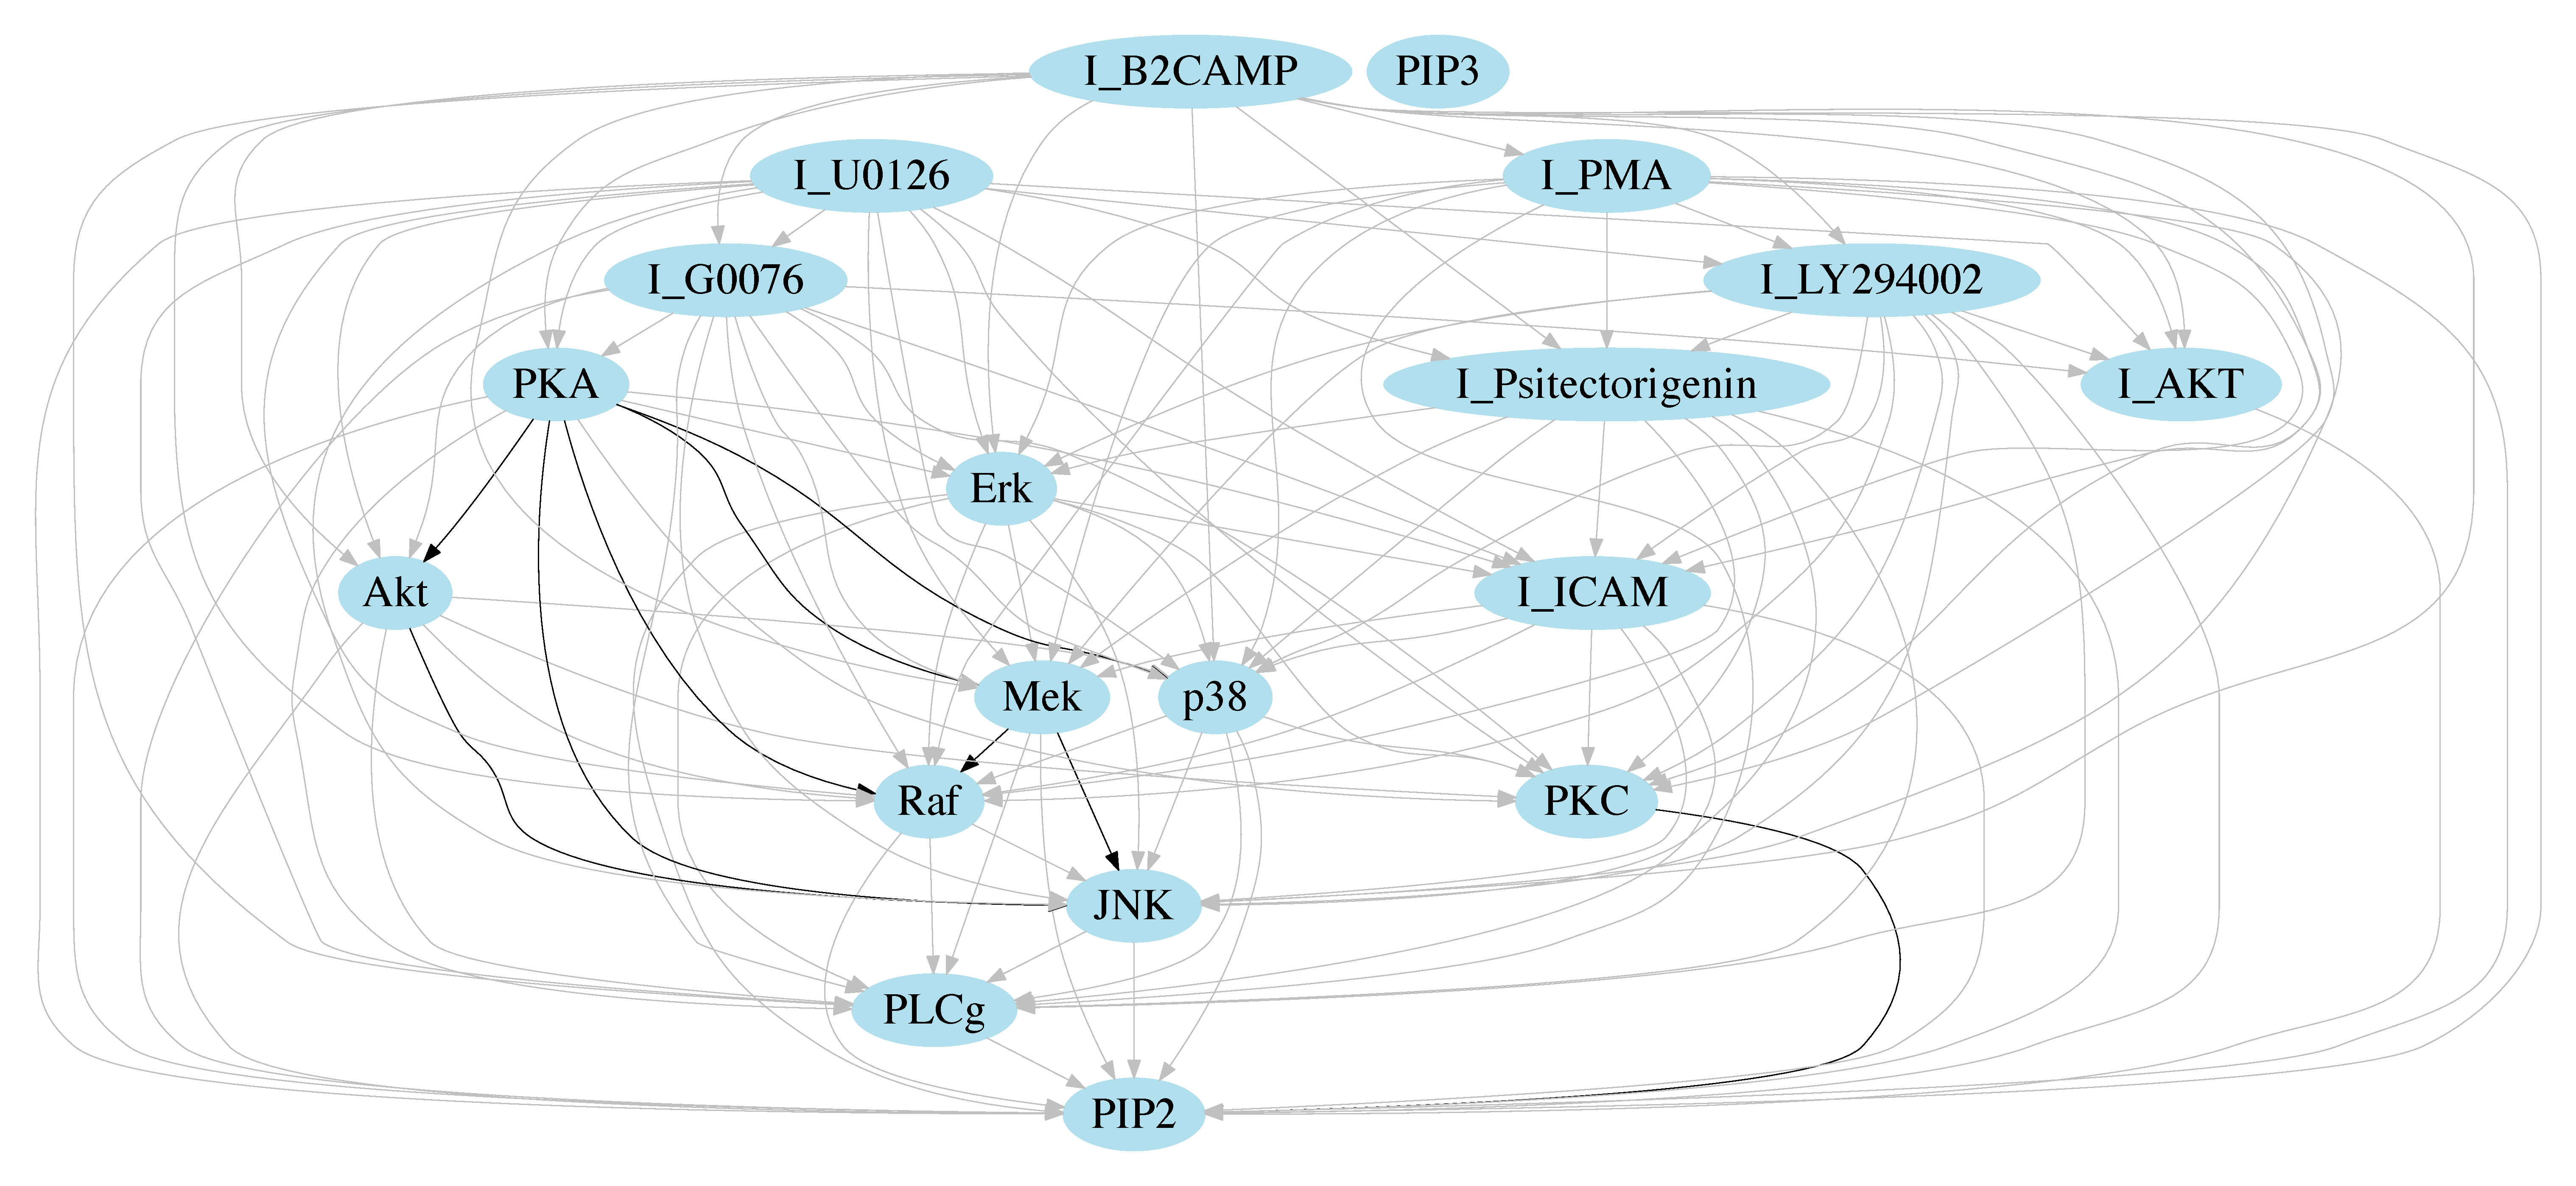
\includegraphics[width=\textwidth]{additional/sachsAncGraph_bootstrap0_priorFALSEgfci}
    \caption{Resulting ancestral graph after applying GFCI to Sachs dataset without a prior. The grey lines show relations which only GFCI found and the black lines show relations ACI and GFCI found. \label{fig:sachspagnopriorgfcianc}}
\end{figure}
\begin{figure}[!ht]
    \centering
    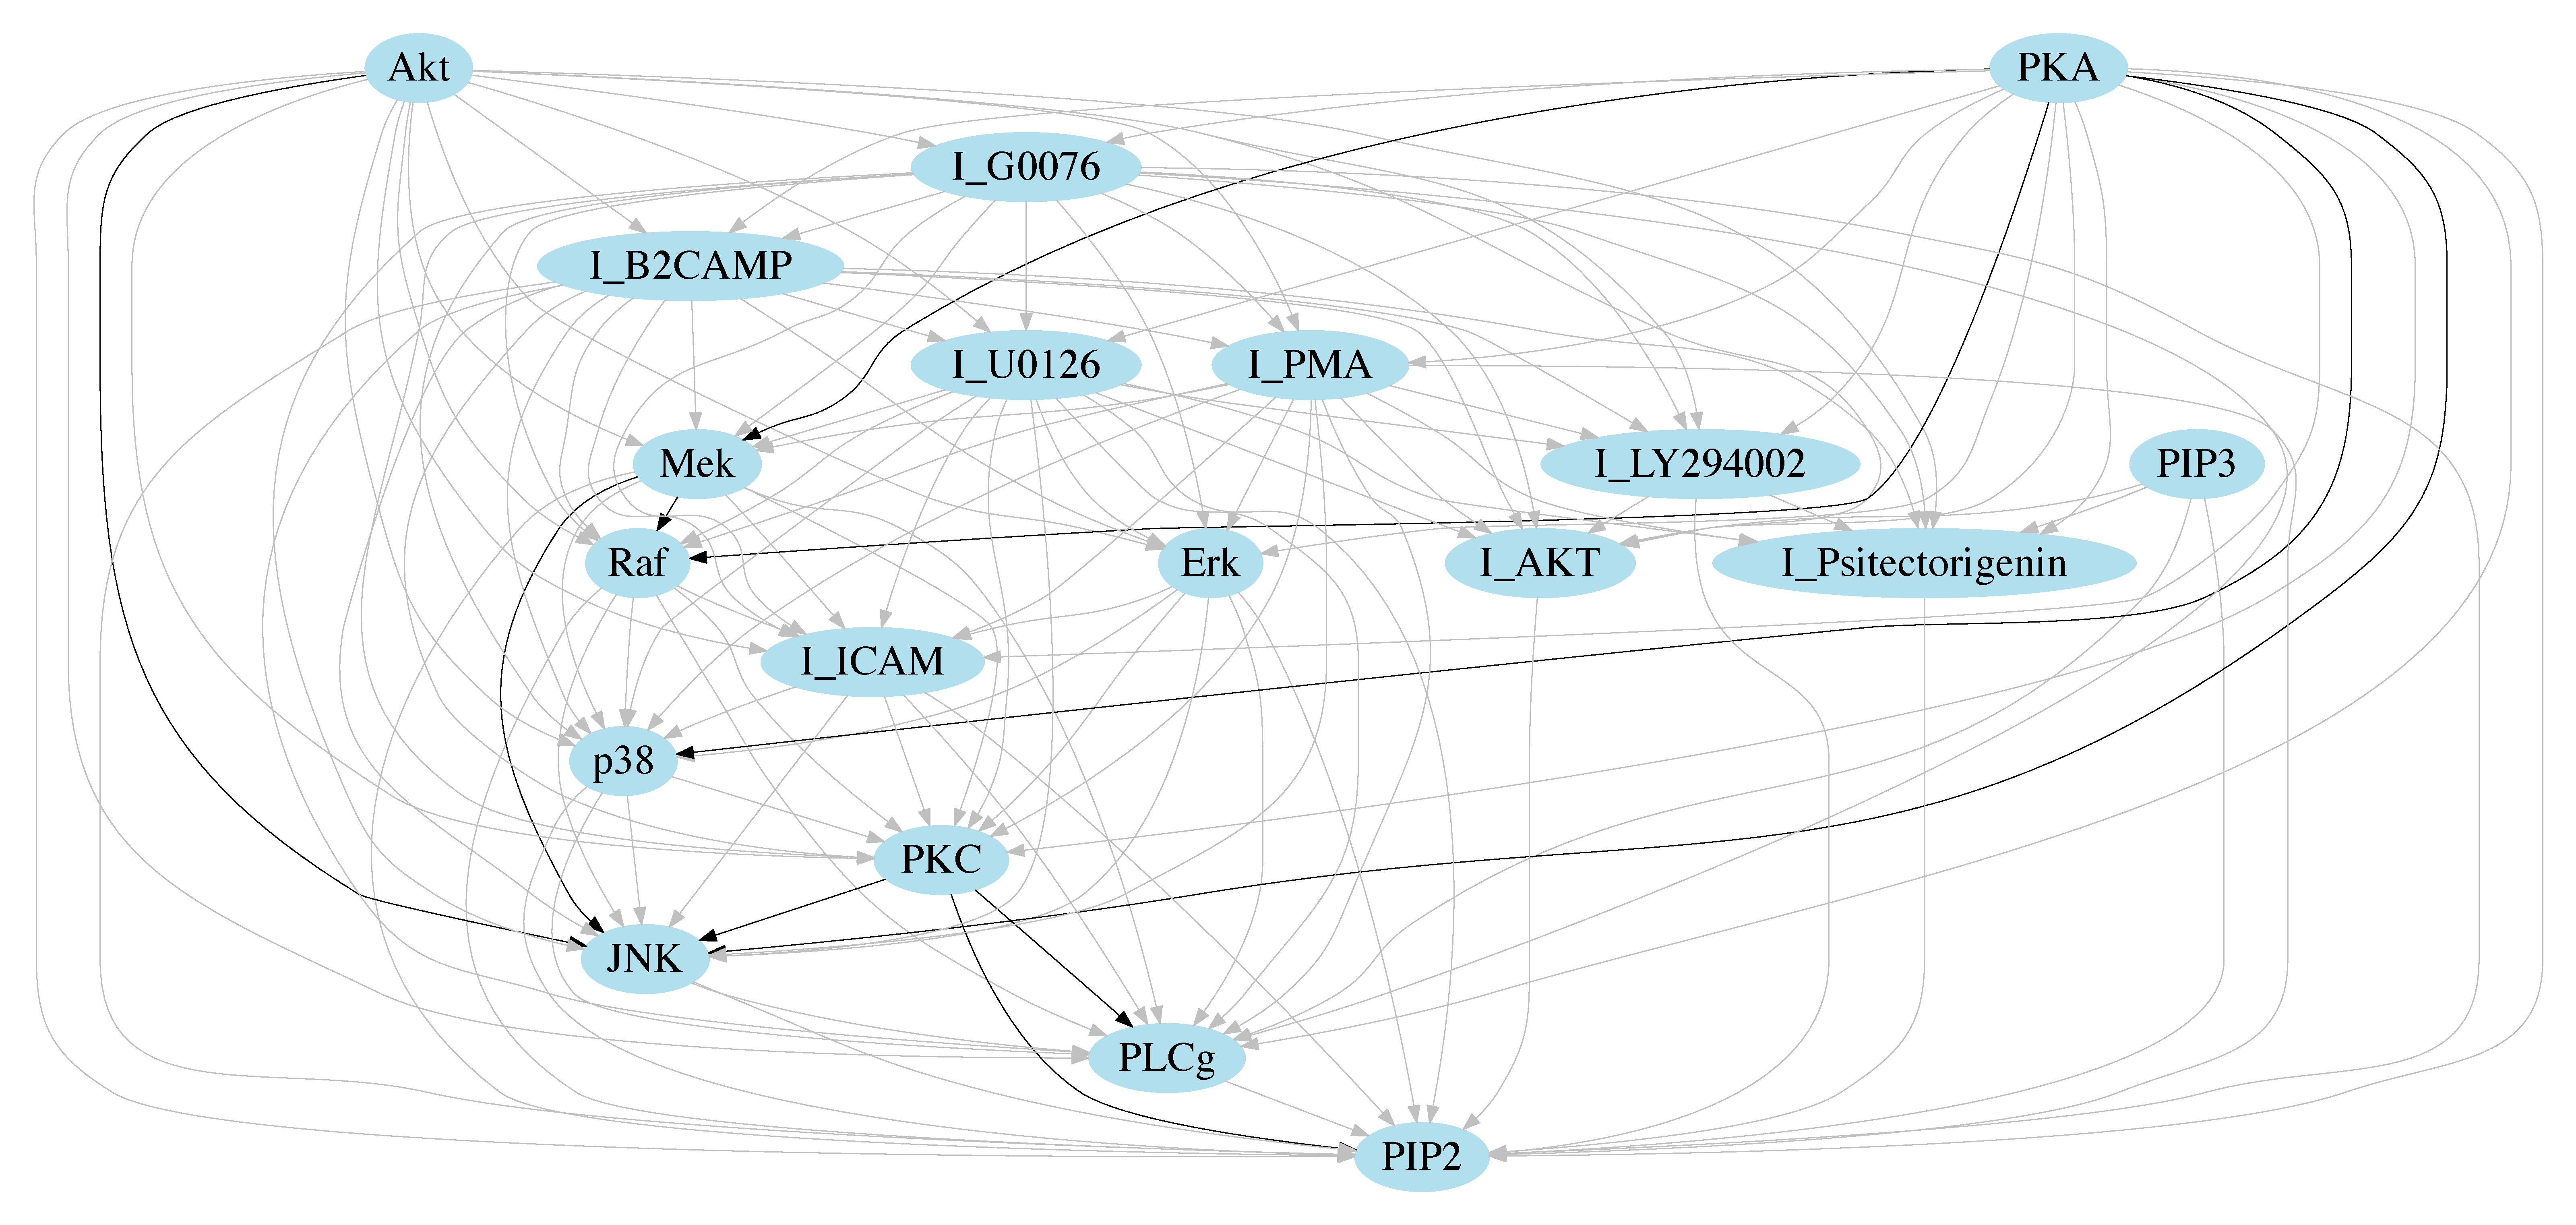
\includegraphics[width=\textwidth]{additional/sachsAncGraph_bootstrap0_priorFALSEfges}
    \caption{Resulting graph after applying FGES to Sachs dataset without a prior. The grey lines show relations which only fges found and the black lines show relations ACI and fges found. \label{fig:sachspagnopriorfgesanc}}
\end{figure}

\newpage % added for layout

\begin{table}[!ht]
\caption{Table from Magliacane et al. \cite{aci} updated to  include GFCI-JCI. This table compares the causal relations found by the consensus model and a number of other causal inference methods. In this table \cite{sachs2005causal}a shows the relations in the consensus model while \cite{sachs2005causal}b shows the reconstruction of this model. Additionally, \cite{MooijHeskes_UAI_13}a shows the top 17 edges in an acyclic setting as described in their paper and \cite{MooijHeskes_UAI_13}b shows the relations for its transitive closure.  The ACI results only include the top 21 ancestral relations. Since GFCI-JCI did not have enough data to be bootstrapped, this is not the case for GFCI-JCI. Instead for GFCI-JCI the relations that are in both GFCI-JCI and any of the other methods in the table will be indicated. Meaning that of the relations found between system variables in Figure \ref{fig:ACIvsGFCIpriorTRUE}, 16 relations are displayed in this table. FGES-JCI is displayed similarly to GFCI-JCI, of the relations found between system variables in Figure \ref{fig:ACIvsFGESpriorTRUE}, 13 relations are displayed in this table.\label{tab:comparisonSachs}}
{\small

\rowcolors{3}{blue!10}{blue!15}
\makebox[\textwidth][c]{\begin{tabular}{l|ccccc|ccccc}
\hline
%
%
  & \multicolumn{5}{|c|}{Direct causal predictions} & \multicolumn{5}{|c}{Ancestral predictions} \\%
%
Edge & \cite{sachs2005causal}a & \cite{sachs2005causal}b & \cite{MooijHeskes_UAI_13}a  & \cite{eaton2007exact} & ICP \cite{ICP_PNAS} & hiddenICP \cite{ICP_PNAS} & \cite{MooijHeskes_UAI_13}b & ACI (top 21)\cite{aci} & GFCI-JCI & FGES-JCI\\
\hline
RAF$\to$MEK   & \cmark & \cmark &         	&
	        &          & \cmark &          & 
& &\\
MEK$\to$RAF   &				&           & \cmark & 
\cmark 	&          & \cmark &  \cmark &
\cmark & \cmark  & \cmark\\
MEK$\to$ERK   & \cmark & \cmark & \cmark & 
            &         &            & \cmark &
\cmark  & &\\
MEK$\to$AKT   & 		   &  		   &  		   & 
            &         &            &  		    &
\cmark& &\\
MEK$\to$JNK   & 		   &  		   &  		   & 
            &         &            &  		    &
\cmark & \cmark & \cmark\\
PLCg$\to$PIP2 & \cmark & \cmark &          &	
\cmark 	& \cmark & \cmark & 		     & 
  & \cmark  & \cmark \\
PLCg$\to$PIP3 &           & \cmark &          &
\cmark 	 &         &           &			 &  
& &\\
PLCg$\to$PKC  & \cmark &           &		  &
\cmark 	 &         &            & 			 &
& &\\
PIP2$\to$PLCg &            &          & \cmark&
			 &\cmark&            & \cmark &
\cmark& &\\
PIP2$\to$PIP3  &            &           &         &
\cmark 	 &         &            &			 &
& &\\
PIP2$\to$PKC   & \cmark  &          &          &
			 &         &             &			  &
& &\\
PIP3$\to$PLCg & \cmark  &           &          & 
			 &         &            &\cmark &
 & \cmark   & \cmark\\
PIP3$\to$PIP2  & \cmark  & \cmark & \cmark &  
            &\cmark& \cmark   & \cmark &
 & \cmark   & \cmark\\
PIP3$\to$AKT  & \cmark   &          &           & 
		     &         &             &          &
& &\\
AKT$\to$ERK   &             &         & \cmark &
            &\cmark& \cmark   &	\cmark &
 & &\\
AKT$\to$JNK   & 		   &  		   &  		   & 
            &         &            &  		    &
\cmark& \cmark &\\
ERK$\to$AKT   &             & \cmark &         & 
\cmark 	 & \cmark & \cmark &				&
& \cmark  & \cmark \\
ERK$\to$PKA   &              &          &          & 
\cmark   &    		 &            	&            &
 & &\\
PKA$\to$RAF   & \cmark    & \cmark &          &
            &          &              &   \cmark &    
\cmark& \cmark &\\
PKA$\to$MEK   & \cmark    & \cmark & \cmark & 
\cmark  &           & \cmark    &  \cmark &
\cmark& &\\
PKA$\to$ERK   & \cmark     & \cmark &          &
          & \cmark &               &  \cmark &
\cmark& \cmark  & \cmark\\
PKA$\to$AKT   & \cmark    & \cmark & \cmark &
\cmark &            & \cmark    &  \cmark &
\cmark& \cmark  & \cmark\\
PKA$\to$PKC   &              &           &           & 
\cmark &            &             &			&
& \cmark &\\
PKA$\to$P38   & \cmark 	  & \cmark  & \cmark &
          &            &             & \cmark &
\cmark& \cmark &\\
PKA$\to$JNK   & \cmark 	  & \cmark  & \cmark &
\cmark &            &             & \cmark &
\cmark& \cmark &\\
PKC$\to$RAF    & \cmark   & \cmark & \cmark  & 
         &              &            &\cmark & 
\cmark& &\\
PKC$\to$MEK   & \cmark & \cmark & \cmark &
\cmark &          &           &  \cmark & 
\cmark& &\\
PKC$\to$PLCg  &              &              & \cmark  &     
         &              &              &\cmark & 
\cmark&  & \cmark\\
PKC$\to$PIP2  &              &              & \cmark  &
         &              &              &  \cmark &          
\cmark&  & \cmark\\
PKC$\to$PIP3   &              &           &           & 
 		&            &             &			&
\cmark& &\\
PKC$\to$ERK   &              &              &   	      & 
       &              &               & \cmark &
\cmark& &\\
PKC$\to$AKT   &              &              & \cmark & 
       &              &               & \cmark &
\cmark& &\\
PKC$\to$PKA   &              & \cmark & \cmark &  
            &              &              & \cmark &
& &\\
PKC$\to$P38   & \cmark & \cmark & \cmark & 
\cmark &              & \cmark &  \cmark & 
\cmark& &\\
PKC$\to$JNK   & \cmark & \cmark & \cmark &
\cmark & \cmark & \cmark &  \cmark &
\cmark &  & \cmark\\
P38$\to$JNK   &              &              &              &
             &              & \cmark &      &
 & \cmark  & \cmark  \\
P38$\to$PKC   &              &              &              & 
            &              & \cmark &          &
& \cmark  & \cmark\\
JNK$\to$PKC   &              &              &              & 
           &              & \cmark &              &
& &\\
JNK$\to$P38   &              &              &              & 
\cmark &              & \cmark &             &
& &\\
\hline
\end{tabular}}

}
\end{table} 
\end{document}
